\documentclass[a4paper,12pt]{article}

% passe en mode large sur la page A4
\usepackage{a4wide}

% document francisé
\usepackage[french]{babel}

% permet la frappe de caractères accentués
\usepackage[utf8x]{inputenc}

\usepackage{bookmark}
\usepackage[T1]{fontenc}
\usepackage{color}
\usepackage{amsmath}
\usepackage{amsfonts}
\usepackage[top=3cm, bottom=3cm, left=2.5cm, right=2.5cm]{geometry}
\usepackage{fancyhdr}
\usepackage{graphicx}
\usepackage{float}
\usepackage{multicol}
\usepackage{multirow}
\usepackage{textcomp}
\usepackage{gensymb}
\usepackage{subcaption}
\usepackage{url}
\usepackage{hyperref}
\usepackage[justification=centering]{caption}

\pagestyle{fancy}

\makeatletter
\newcounter{subsubsubsection}[subsubsection]
\renewcommand\thesubsubsubsection{\@roman\c@subsubsubsection}
\newcommand\subsubsubsection{\@startsection{subsubsubsection}{4}{\z@}%
                                     {-3.25ex\@plus -1ex \@minus -.2ex}%
                                     {1.5ex \@plus .2ex}%
                                     {\normalfont\small\bfseries}}
\newcommand*\l@subsubsubsection{\@dottedtocline{3}{5.2em}{1em}}
\newcommand*{\subsubsubsectionmark}[1]{}
\setcounter{secnumdepth}{4}
\makeatother

% individualisation des paramètres de la page
%\parskip7pt
\setlength{\topmargin}{-10mm}
%\setlength{\textheight}{250mm}

%En-tête
\renewcommand{\headrulewidth}{0.3pt}
\fancyhead[C]{}
\fancyhead[L]{L1 CMI OPT/IM -- ICM -- INA}
\fancyhead[R]{Projet d'initiation à l'ingénierie}
\setlength{\headheight}{15pt}
%Pied de page
\renewcommand{\footrulewidth}{0.3pt}
\fancyfoot[L]{2020-2021}
\fancyfoot[C]{\textbf\small{\thepage}}
\fancyfoot[R]{\footnotesize{Rapport final}}

\begin{document}

%
% -------------------------------------------------------------------------------------------
%
\begin{figure}[H]
  \centering
  \includegraphics[width=0.3\textwidth]{univ nantes.png}
\end{figure}

\begin{center}
	{\large {L1 CMI -- Projet d'initiation à l'ingénierie}} \\
	\vspace{6cm}
  {\Large \textbf{Conception et réalisation de la plateforme de Stewart} \\
	\vspace{2mm}
	Etudiants : Baptiste Deshayes, Malo Le Bourlout, Simon Massonnaud, Eliott Petiteau

    Encadrants : Rabah Bouzidi et  Nicolas Dupont-Bloch\\
	\vspace{9cm}	
	Janvier - mai 2021} \\
	\vspace{3mm}
	
\end{center}

\newpage

\tableofcontents

\newpage
%
% ====================================================================
%
\section{Introduction}

La plateforme de Stewart est un positionneur hexapode composé d’un plateau fixe et d’un plateau mobile. 
Ces deux plateaux sont maintenus à l’aide de six actionneurs linéaires qui s’apparentent à des vérins \textit{(nous les nommerons indifféremment aussi dans le rapport bielles ou tendeurs)}. Le but de cette plateforme est de s'adapter à tous les mouvements possibles.
Le plateau supérieur peut se déplacer selon les trois axes (x, y et z), il peut également s’incliner suivant trois axes. 
Grâce à ces six bielles pouvant indépendamment changer de longueur, la plateforme supérieure peut former n’importe quel plan, elle est juste limitée par la longueur des bielles. 
Il faut actionner les six bielles qui relient les deux plateaux pour faire varier leur longueur et ainsi changer l’orientation de la plateforme. 
Chaque position de la plateforme supérieure correspond à une seule combinaison des six longueurs.


\begin{figure}[H]
  \centering
  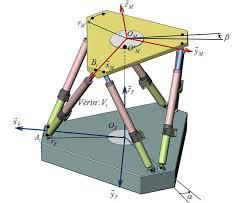
\includegraphics[width=0.4\textwidth]{schema plateforme.png}
  \caption{Illustration de la plateforme de Stewart}
\end{figure}

\medskip

Cette plateforme peut avoir de nombreux usages. 
Elle peut être utilisée comme base pour une cabine de simulateur de vols, pour la conception de grues, la recherche
sous-marine ou encore pour les télescopes. 
Effectivement, la nature de ces activés nécessite un positionnement très précis et la plateforme de
Stewart répond à ce besoin. 
D’un coté, cette plateforme est une avancée technologique dans de nombreux secteurs car elle joue le rôle de simulateur. Elle permet donc d’anticiper des comportements sans avoir à réaliser des
tests en conditions réelles. Et d’un autre coté, cette plateforme a permis une excellente précision par rapport à ce qu'il était possible de réaliser auparavant.

\medskip

Notre projet a pour but d’équiper un télescope de Newton. 
Le principe de ce télescope est assez simple, en forme de tube. 
Les rayons lumineux rentrent à une extrémité du tube et sont projetés sur un miroir concave afin de diriger les rayons vers un autre miroir en face du premier. 
C’est ce deuxième miroir que nous regardons avec notre oeil sur le coté du tube ; ce miroir est incliné afin de changer la direction des rayons lumineux et de les faire parvenir à notre oeil. 
Pour avoir l’image la plus nette possible, il faut limiter le nombre de miroirs. 
Nous pouvons donc imaginer un télescope ayant juste le premier miroir et mettre notre oeil en face de ce dernier afin d’avoir une image la plus nette possible. 
Le problème est que notre tête va créer un zone d’obstruction trop importante. 
En effet, notre tête va éclipser une partie du ciel que nous voulons observer. 
Le but est donc de réduire au maximum cette zone d’obstruction. 
On utilise pour cela une caméra car elle est bien moins volumineuse que notre tête. 
On l’utilise également pour capter ces images et en prendre un cliché. 
Cette caméra nécessite d’être fixée au télescope et d’être à bonne distance du miroir. 
Il faut que la caméra soit à bonne distance afin d’être exactement sur le point focal, c’est la distance à laquelle tous les rayons réfléchis par le miroir concave se rejoignent et forment une image nette. 
Pour s’assurer que la caméra soit à la bonne distance, nous allons utiliser la plateforme de Stewart. 
Nous fixerons la caméra au centre du plateau supérieur et le plateau bas sera relié au télescope. 
Nous pourrons alors ajuster la position de la caméra très précisément afin d’être à la bonne distance focale. 

\begin{figure}[H]
    \centering
    \begin{subfigure}[]{0.4\textwidth}
        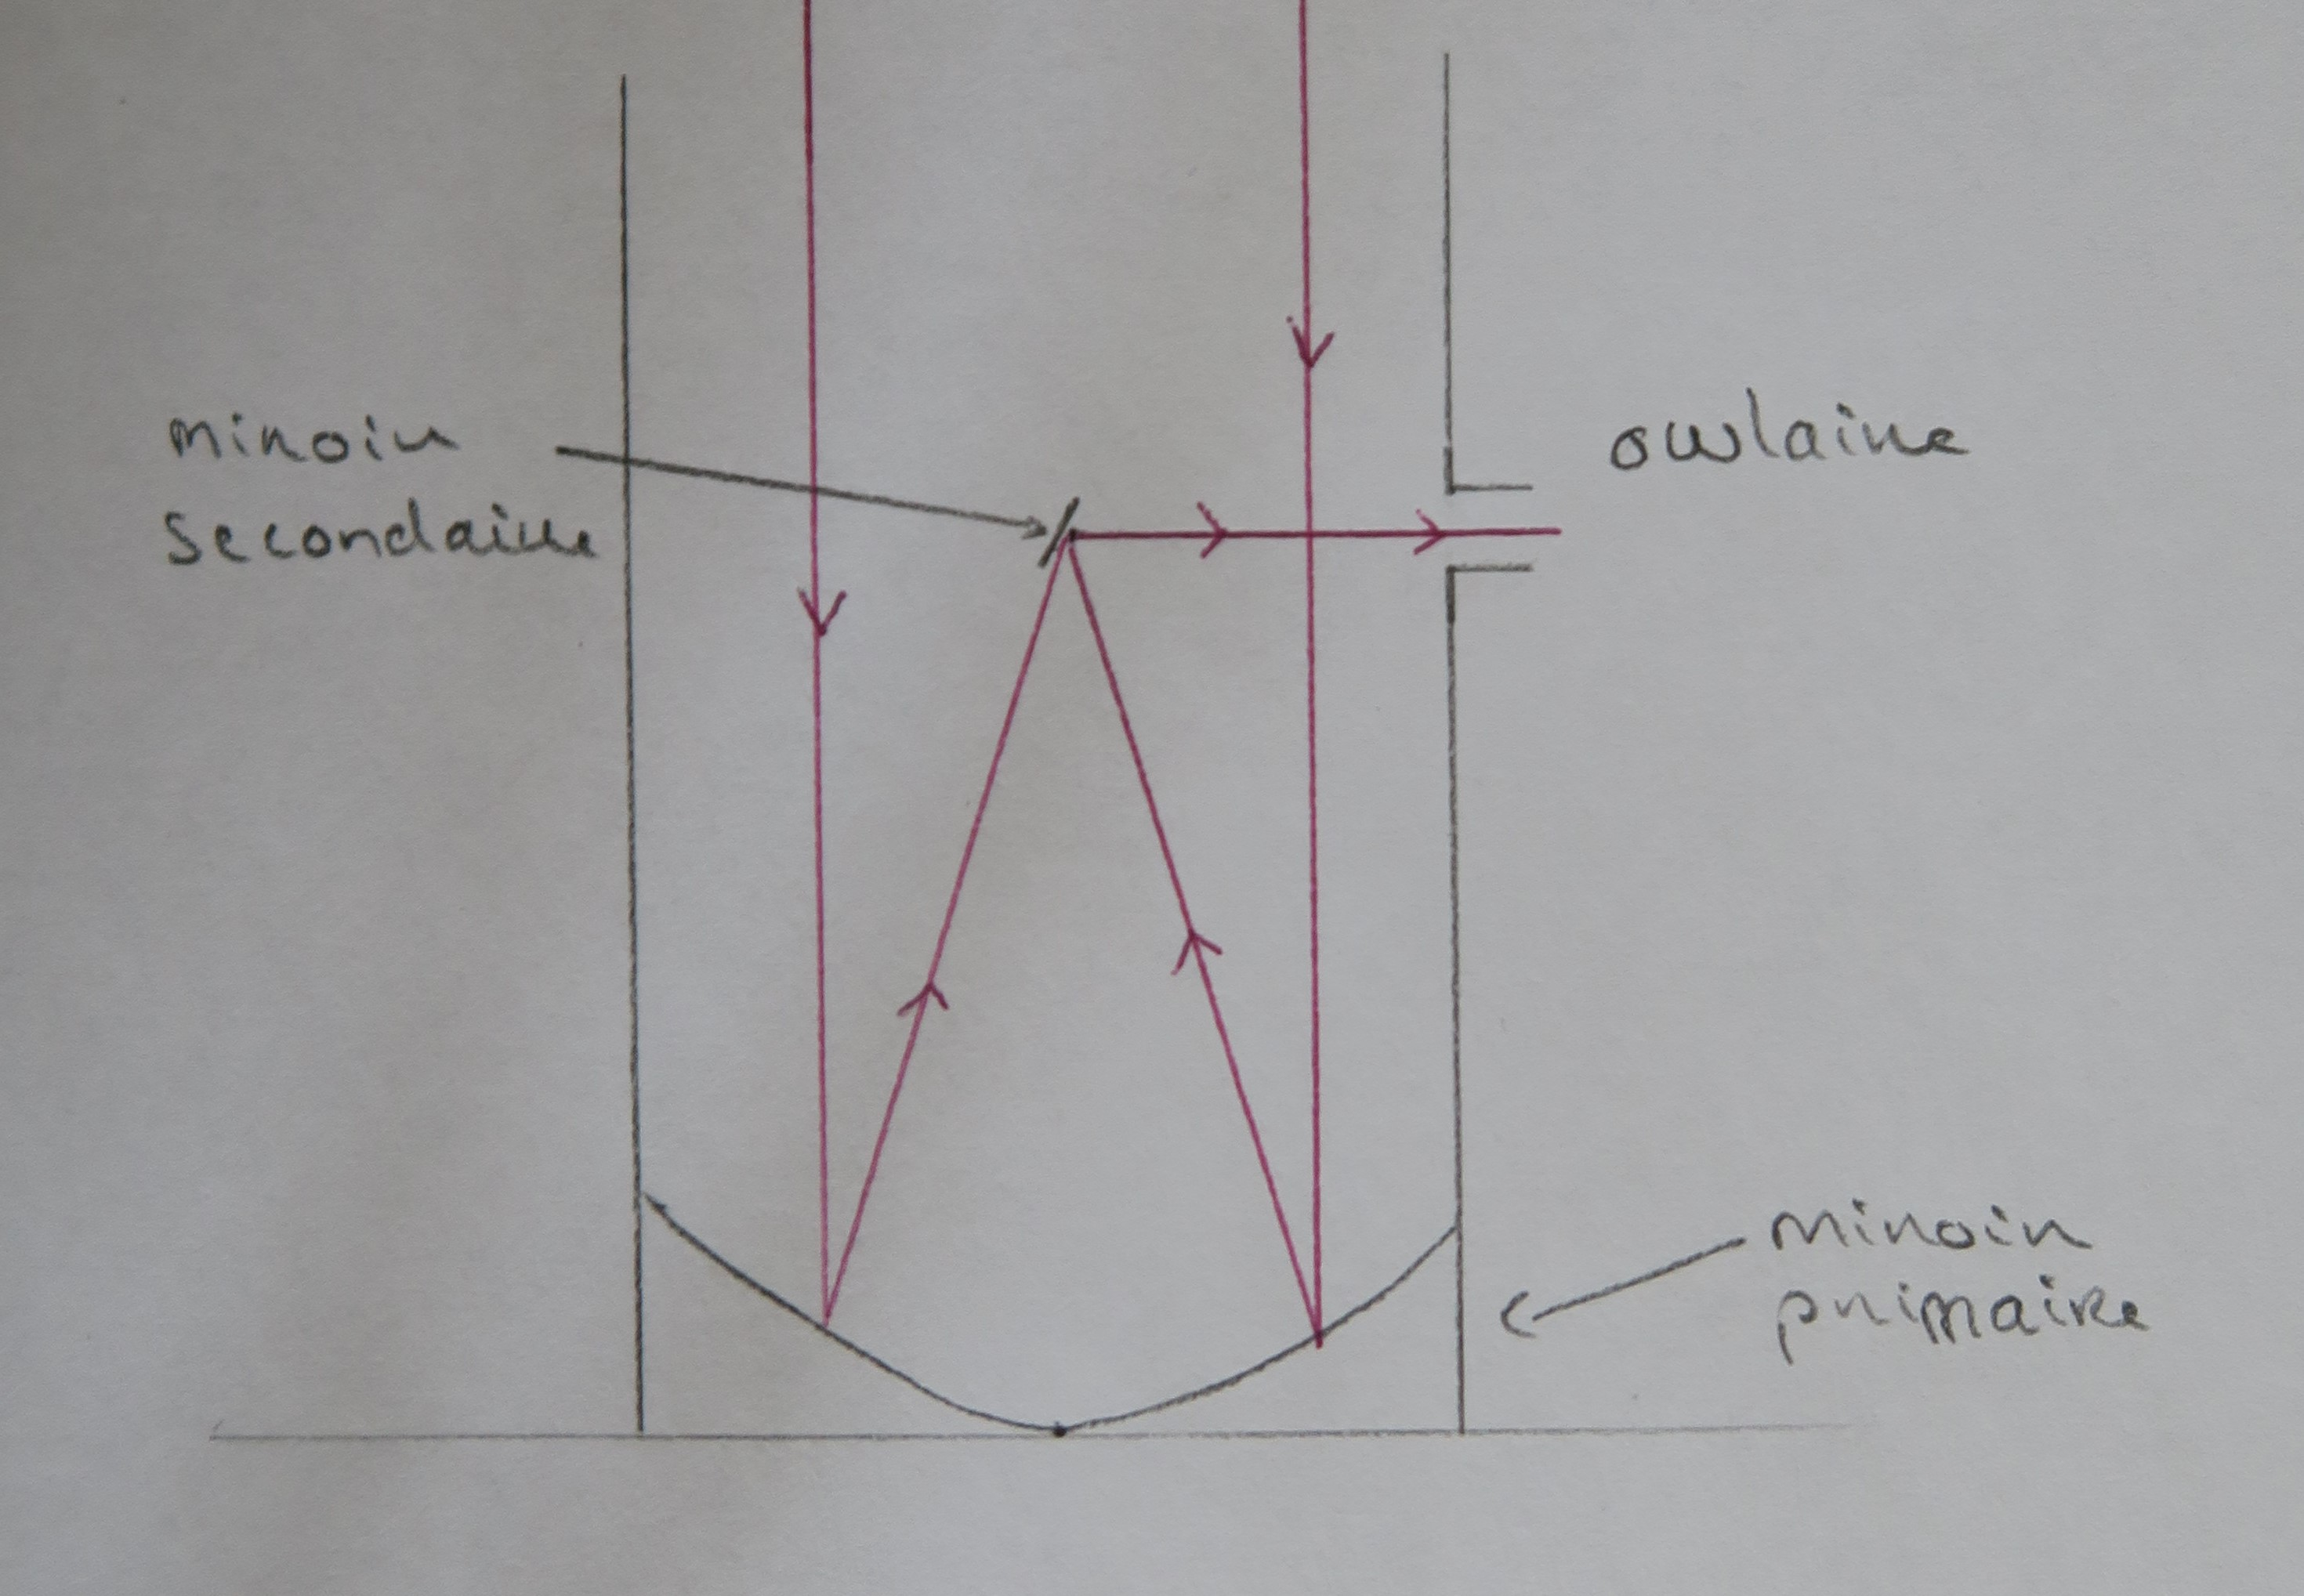
\includegraphics[width=\textwidth]{dessin telescope.jpg}
    \end{subfigure}
    \begin{subfigure}[]{0.4\textwidth}
        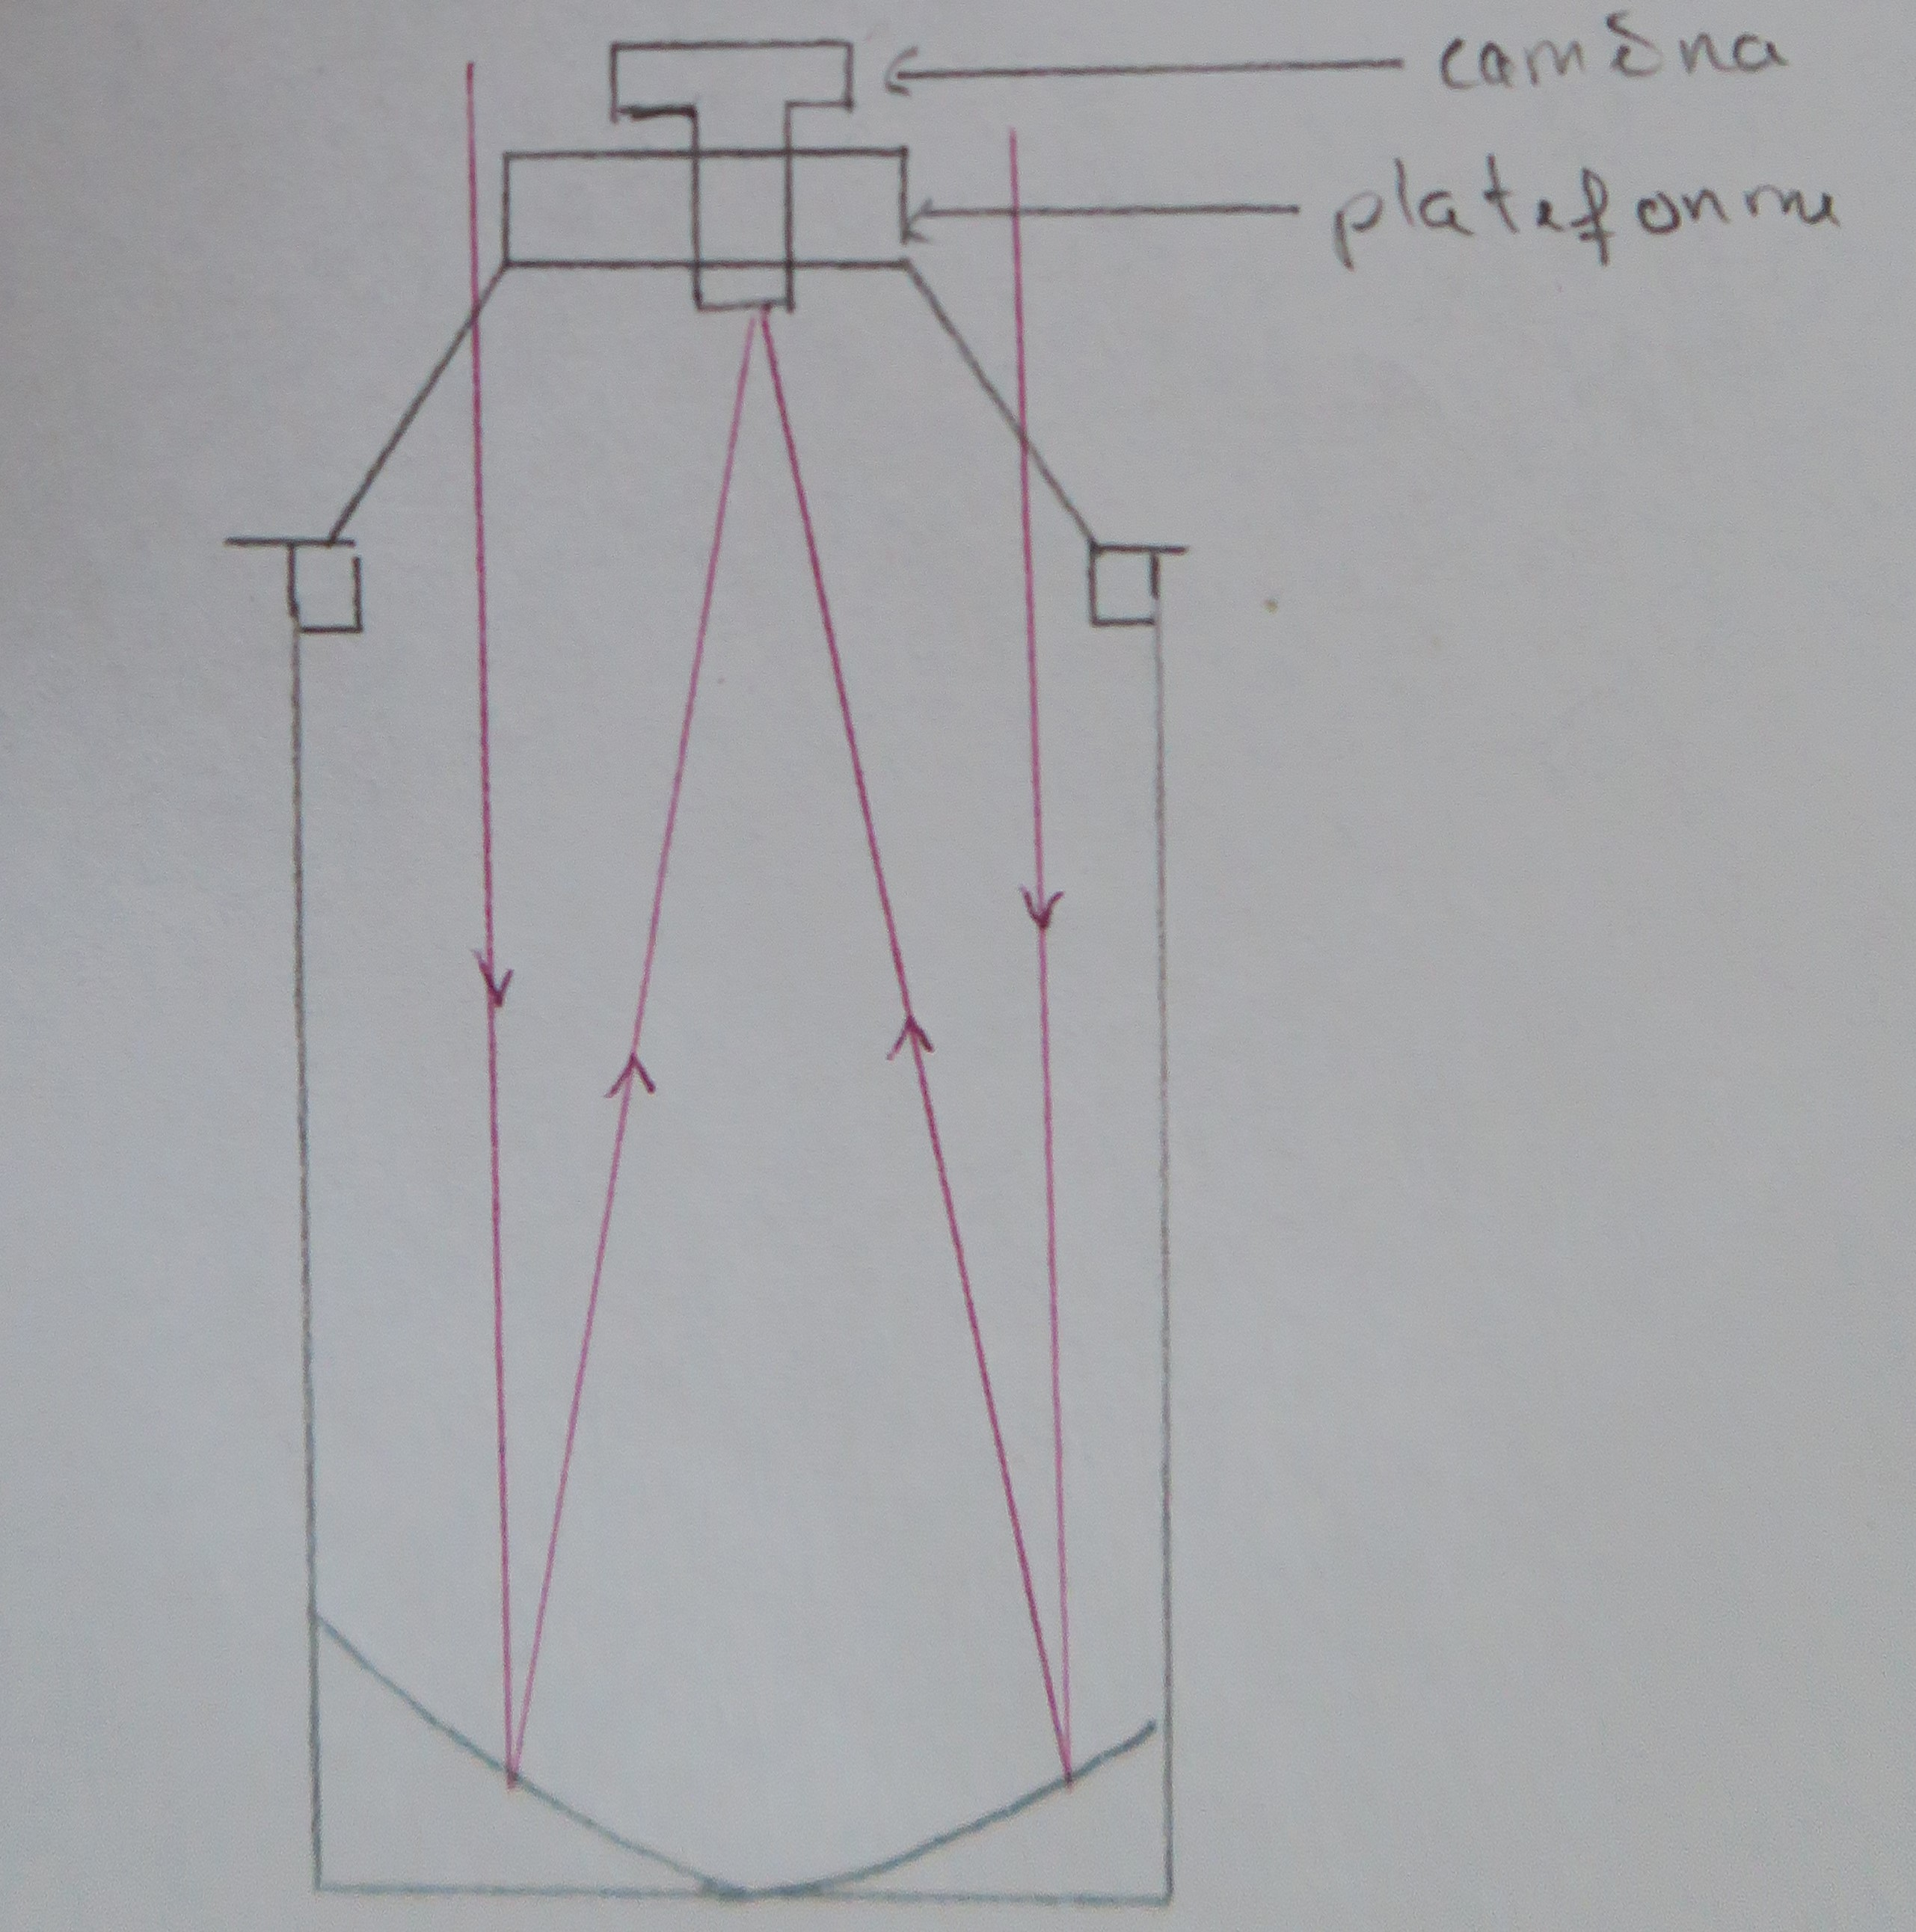
\includegraphics[width=\textwidth]{dessin telescope avec plateforme.jpg}
    \end{subfigure}
    \caption{Schéma du télescope de Newton avec et sans la plateforme de Stewart}
\end{figure}




\medskip

La temporalité du projet s'est séquencée en cinq temps : \\
-échanges/discussions avec notre encadrant sur les créneaux de cours pour guider l'avancement de notre projet ; \\
-échanges/discussions entre nous quatre pour mettre en commun et confronter nos temps de travail individuel, décider des options de conception et modélisation à prendre et de la marche à suivre pour engager les différentes étapes du projet ; \\
-temps de regroupement pour mettre en application ( = montage de la plateforme) ; \\
-finalisation de la réalisation de la plateforme ( = ajustements du montage) durant les vacances de printemps ; \\
-co-rédaction du rapport final.

\newpage

\section{Problématique}


Le problème traité dans ce projet est la réalisation d'une plateforme de Stewart qui se décompose en quatre étapes : \\
- la conception de celle-ci, en accord avec les dimensions requises pour sa future utilisation (ajuster la position d'une caméra sur un télescope de Newton), à l'aide d'un logiciel de modélisation 3D (ici FreeCAD) ; \\
- la création d'un tableur permettant de calculer et d'optimiser les longueurs des actionneurs linaires en fonction de la position voulue de la plateforme ; \\
- l'impression en 3D des pièces modélisées, l'achat des pièces de jonction et des actionneurs linéaires ; \\
- et enfin l'assemblage de la plateforme.

\medskip

Afin de créer une plateforme de Stewart, il nous est nécessaire de connaître  la cinématique de la plateforme et comment elle est affectée par les variations de longueur des six éléments linéaires qui la composent.
Il nous faut donc établir les différentes équations permettant de retrouver la longueur de chacun des éléments linéaires en fonction des mouvements de translation et de rotation que nous souhaitons effectuer. 

\medskip

La plateforme de Stewart est un outil dont l'utilisation est déjà répandue dans de multiples domaines, possédant donc diverses analyses sur son comportement, souvent abordées par cinématique inversée. 
Ses applications en robotique ont notamment fourni des analyses d'un point de vue électronique de la plateforme, ainsi que de sensibilité de ses mouvements dans le cadre de différents usages tel l'aéronautique.

\newpage

\section{Mise en oeuvre de la plateforme}

Dans cette partie, nous allons voir comment résoudre le problème posé. 
Cette résolution passe par deux grandes étapes.
Dans un premier temps, nous devons réaliser le modèle mathématique qui permet de contrôler la plateforme, nous avons pour cela créé un tableur Excel. Dans un second temps, nous devons créer la plateforme en elle-même, c'est-à-dire la modéliser pour qu'elle réponde à toutes les contraintes amenées par et pour sa future utilisation.

\subsection{Formulation cinématique}
	
L’objectif de ce tableur est de créer un modèle mathématique théorique et précis pour contrôler le fonctionnement de la plateforme de Stewart. 
Nous supposons, pour créer ce modèle, que la plateforme s’apparente à deux disques reliés par six axes et espacés d’une hauteur fixée quand l’appareil est au repos. 
Nous avons séparé notre travail en étudiant d’un côté, la partie basse de la plateforme et de l’autre, sa partie haute.

\subsubsection{Partie basse de la plateforme}

Intéressons-nous à la partie basse. 
Nous supposons que le disque qui la constitue est divisé en trois. C’est-à-dire que chaque point est séparé de cent vingt degrés en prenant des points aux angles 0\degree, 120\degree et 240\degree. 
Ensuite, nous fixons un écart par rapport à ces angles qui peut être choisi par l’utilisateur. 
Nous appelons cet écart \og delta thêta \fg. Il représente la position des six points d’accroches de nos axes. 
De chaque côté des trois angles principaux, de 0\degree, 120\degree et 240\degree, nous ajoutons la valeur de \og delta thêta \fg \ pour trouver un premier point et nous la retirons pour trouver un deuxième point. 
Prenons un exemple pour illustrer le fonctionnement de ce \og delta thêta \fg . 
Prenons-le de 30\degree et prenons le point à l’angle 0\degree. Comme expliqué, nous trouvons donc un point à 30\degree et un autre à -30\degree ou 330\degree. 
Une fois ces points déterminés, nous calculons leur valeur en radians. 
De ces valeurs en radians, nous pouvons déterminer les coordonnées des points selon les axes x, y et z. 
Pour la coordonnée selon l’axe z, elle vaut 0 car nous sommes sur la partie basse de la plateforme. 
Pour les coordonnées selon les axes x et y, nous appliquons respectivement la fonction cosinus et sinus à chaque angle tout en multipliant par le rayon de la plateforme. 
Nous connaissons donc les coordonnées des six points bas de la plateforme.


\begin{figure}[H]
  \centering
  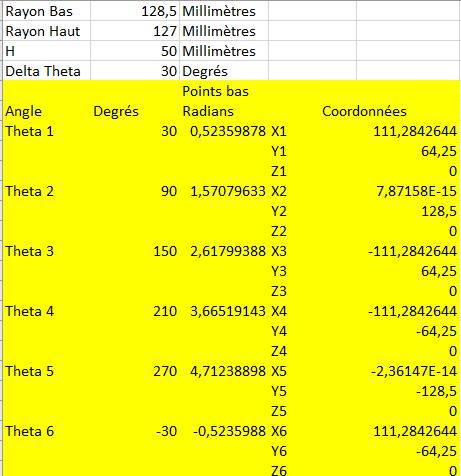
\includegraphics[width=0.5\textwidth]{tableur points bas.jpg}
  \caption{Tableur points bas}
\end{figure}

\subsubsection{Partie haute de la plateforme}

Intéressons-nous maintenant à la partie haute de la plateforme. 
Nous supposons que ce disque est parfaitement parallèle à la partie basse et que ces deux disques sont séparés d’une hauteur fixée nommée \og h \fg . 
Nous supposons là aussi que le disque est séparé en trois points selon les mêmes positions que pour la partie basse de la plateforme. 
Ces trois points représentent les points d’arrivées des six axes qui partent de la partie basse. 
Nous calculons, suivant le même raisonnement que précédemment, les coordonnées de ces points selon les axes x, y et z, à une différence près. 
En effet, comme nous étudions maintenant la partie haute de la plateforme, nous nous trouvons à une hauteur \og h \fg \ de la partie basse. 
Ainsi la coordonnée selon l’axe z vaut h.  
Nous connaissons maintenant les coordonnées théoriques de chacun des trois points de la partie haute de la plateforme. 
Ces coordonnées théoriques seront modifiées par la suite lors de l’utilisation de la plateforme. 
Ces nouvelles coordonnées seront appelées \og coordonnées ajustées \fg . 
Au début, nous initialisons ces coordonnées ajustées avec les coordonnées théoriques pour continuer de réaliser le modèle mathématique.  
Nous calculons ensuite les écarts entre les points AB, AC et BC selon les axes x, y et z. 
Pour cela, nous calculons la différence entre les coordonnées. 
Ensuite, à partir de ces distances entre tous les points, nous pouvons calculer la norme des trois vecteurs que sont $\overrightarrow{AB}$, $\overrightarrow{AC}$, et $\overrightarrow{BC}$. Nous définissons également une valeur cible pour la norme des vecteurs. 
Cette valeur vaut racine de trois multipliée par le rayon de la plateforme haute. 

\begin{figure}[H]
  \centering
  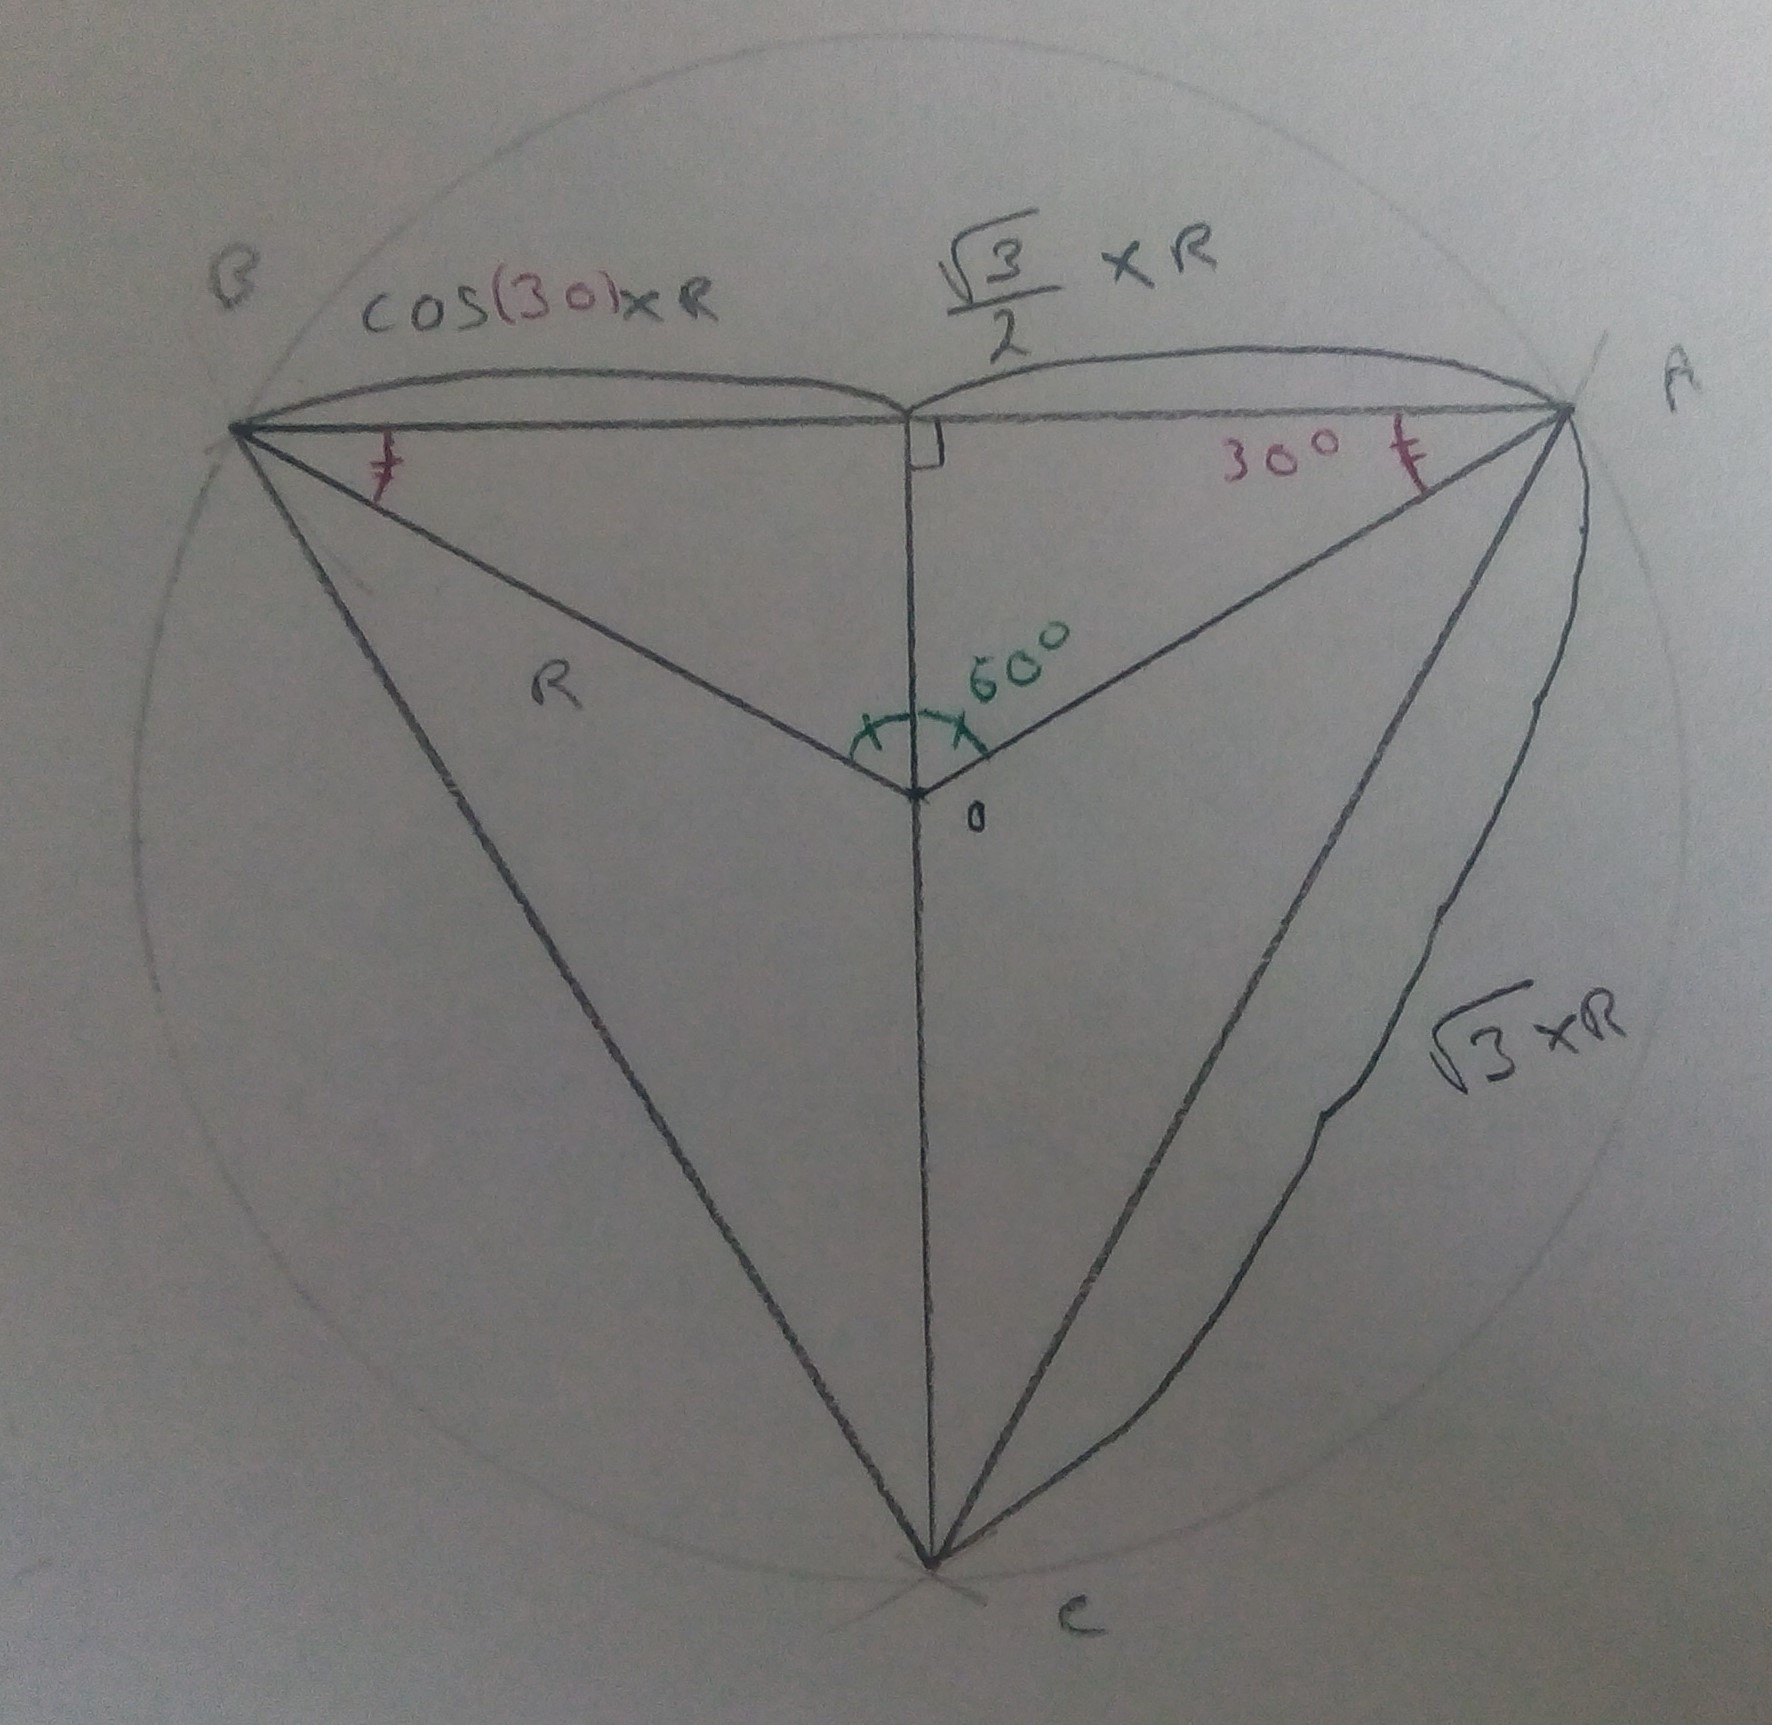
\includegraphics[width=0.4\textwidth]{schema explication.jpg}
  \caption{Schéma d'explication pour le calcul de la norme des vecteurs}
\end{figure}

Nous calculons ensuite le produit vectoriel de $\overrightarrow{AB}$ par $\overrightarrow{AC}$ ainsi que sa norme car ce calcul va intervenir plus tard dans le tableur. 
Nous créons également une colonne qui contiendra les coordonnées ajustées des points hauts, mais nous y reviendrons plus tard. En effet, cette colonne n'intervient qu'à la toute fin du tableur.


\begin{figure}[H]
  \centering
  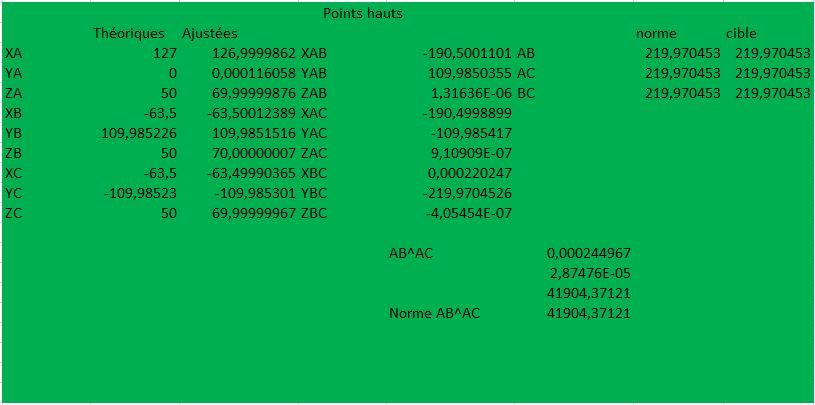
\includegraphics[width=0.7\textwidth]{tableur points hauts.jpg}
  \caption{Tableur points hauts}
\end{figure}

\subsubsection{Longueurs des bielles qui relient les plateaux}

Maintenant que nous connaissons les coordonnées de tous les points d'accroches, nous pouvons raisonner sur la longueur des bielles, ce qui est l'objectif principal, c'est-à-dire déterminer leurs longueurs en fonction de la position voulue. 
Pour chacune des bielles, nous calculons sa longueur à partir des coordonnées théoriques de chaque point. 
Nous calculons la différence entre la coordonnée du point haut et celle du point bas selon chaque axe. 
Nous élevons ces différences au carré puis nous ajoutons les valeurs pour chaque axe et nous en prenons la racine carrée afin de connaître la longueur de la bielle. 
Étant donné que nous avons six bielles, nous répétons l'opération pour chacune d'elles. 
Dans cette partie du tableur, nous créons une colonne appelée \og longueurs ajustées \fg . 
C'est dans celle-ci que nous pourrons lire la valeur de la longueur qu'il faudra donner à chaque bielle pour pouvoir placer la plateforme à la position voulue. 
Nous créons, pour clôturer cette partie du tableur, une dernière colonne dans laquelle nous pouvons lire l'écart de longueur delta entre les bielles à l'origine et la longueur de chaque bielle pour la position voulue.


\begin{figure}[H]
  \centering
  \includegraphics[width=0.5\textwidth]{tableur barres.JPG}
  \caption{Tableur bielles}
\end{figure}

\subsubsection{Valeurs cibles à obtenir}

Voyons maintenant la dernière partie du modèle mathématique, celle qui nous permet de donner la position souhaitée de la plateforme et qui permet de déterminer la longueur à donner aux bielles. Pour commencer, nous déterminons la position du point au centre du plateau haut. 
Nous appelons ce point \og G \fg. 
La coordonnée en x de ce point est la moyenne des coordonnées ajustées des points hauts selon cet axe. 
Nous suivons la même procédure pour chacun des axes. 
Nous créons ensuite une partie dédiée au centre de masse de la plateforme haute. 
Pour déterminer la valeur selon x de ce centre de masse, nous effectuons simplement la division de la coordonnée en x du produit vectoriel de $\overrightarrow{AB}$ par $\overrightarrow{AC}$ par sa norme. 
Nous répétons le même calcul pour les deux autres axes. 
Ensuite, nous créons une colonne où nous entrons les valeurs \og cibles \fg. 
Ces valeurs correspondent à la position que nous voulons donner au point qui est au centre de la plateforme, le point G. 
Nous pouvons également donner une valeur cible aux coordonnées en x et y du centre de masse. Ensuite, nous calculons les écarts entre la valeur cible et la valeur théorique des coordonnées du point G et du centre de masse. 
Nous élevons ces écarts au carré pour n'avoir que des valeurs positives. 
Nous sommons ensuite tous ces écarts, ce sera notre fonction \og coût \fg. 
Nous faisons également le choix de pouvoir donner des coefficients à ces valeurs pour agir plus ou moins sur le centre de masse ou les coordonnées du point G.

\begin{figure}[H]
  \centering
  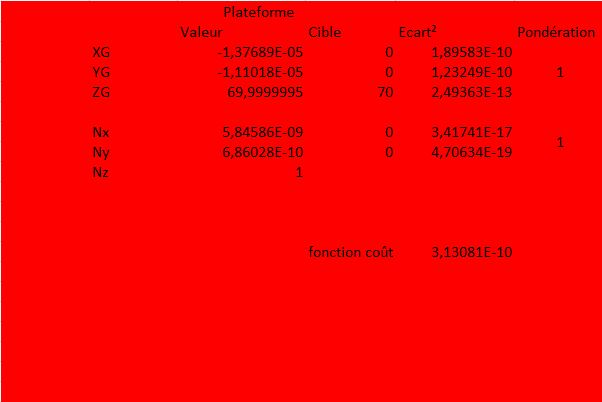
\includegraphics[width=0.7\textwidth]{tableur valeurs cibles.jpg}
  \caption{Tableur valeurs cibles}
\end{figure}

\subsubsection{Fonction solveur}

Maintenant nous allons voir comment nous obtenons les longueurs ajustées des bielles. 
Nous utilisons pour cela la fonction solveur du tableur Excel. 
Le but est de minimiser la fonction coût, qu'elle soit la plus proche possible de zéro. 
Nous avons également une contrainte : il faut que les normes des vecteurs $\overrightarrow{AB}$, $\overrightarrow{AC}$, et $\overrightarrow{BC}$ soient égales ou du moins les plus proches possibles des normes cibles de ces vecteurs. 
Nos variables sont les coordonnées ajustées des points hauts. 
En les modifiant, nous calculons les longueurs ajustées des bielles qui sont donc les longueurs finales à donner aux bielles pour avoir la plateforme à la position souhaitée. 
En appliquant donc la fonction solveur, nous pouvons pour chaque position souhaitée obtenir la longueur à donner aux bielles.


\begin{figure}[H]
  \centering
  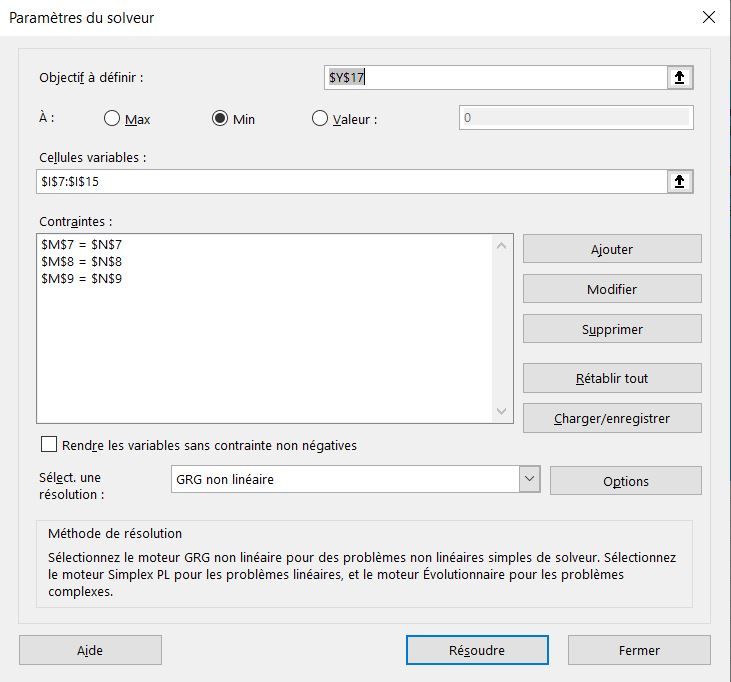
\includegraphics[width=0.5\textwidth]{tableur solveur.jpg}
  \caption{Tableur solveur}
\end{figure}

\subsection{Réalisation de la plateforme}
La plateforme est composée de deux plateaux, un plateau inférieur et un plateau supérieur. 
Les attentes de ces deux plateaux sont différentes donc leur apparence et leur modélisation le seront aussi.

\subsubsection{Contraintes de la plateforme}

\subsubsubsection{Plateau inférieur}

Le plateau inférieur a quelques contraintes,
notamment cette première : obstruer le moins possible le passage de la lumière qui doit arriver jusqu’au télescope. 
Pour cela nous décidons de l'évider (ne modéliser que les bords extérieurs du cercle). 
Le plateau doit aussi s’emboîter parfaitement dans le tube du télescope sans bouger et ainsi garder l’ensemble de la plateforme stable. 
Nous décidons donc de créer une bordure de quelques millimètres, ainsi une partie s’imbriquera parfaitement dans le télescope et l’autre sera trop grande empêchant la plateforme de rentrer entièrement. 
Enfin, nous devons modéliser six trous à intervalles réguliers qui faciliteront le perçage après impression, intervalles choisis au préalable via les calculs mathématiques précédemment exposés et selon les besoins de la plateforme. 
Ces trous serviront plus tard à visser les tendeurs, il faut donc les modéliser en gardant bien cette idée à l’esprit. C’est pourquoi nous les modélisons sur la plus grande bordure (extérieure au tube du télescope) pour éviter une quelconque gêne des tendeurs à la pose ou à la stabilité de la plateforme dans le tube.

\begin{figure}[H]
  \centering
  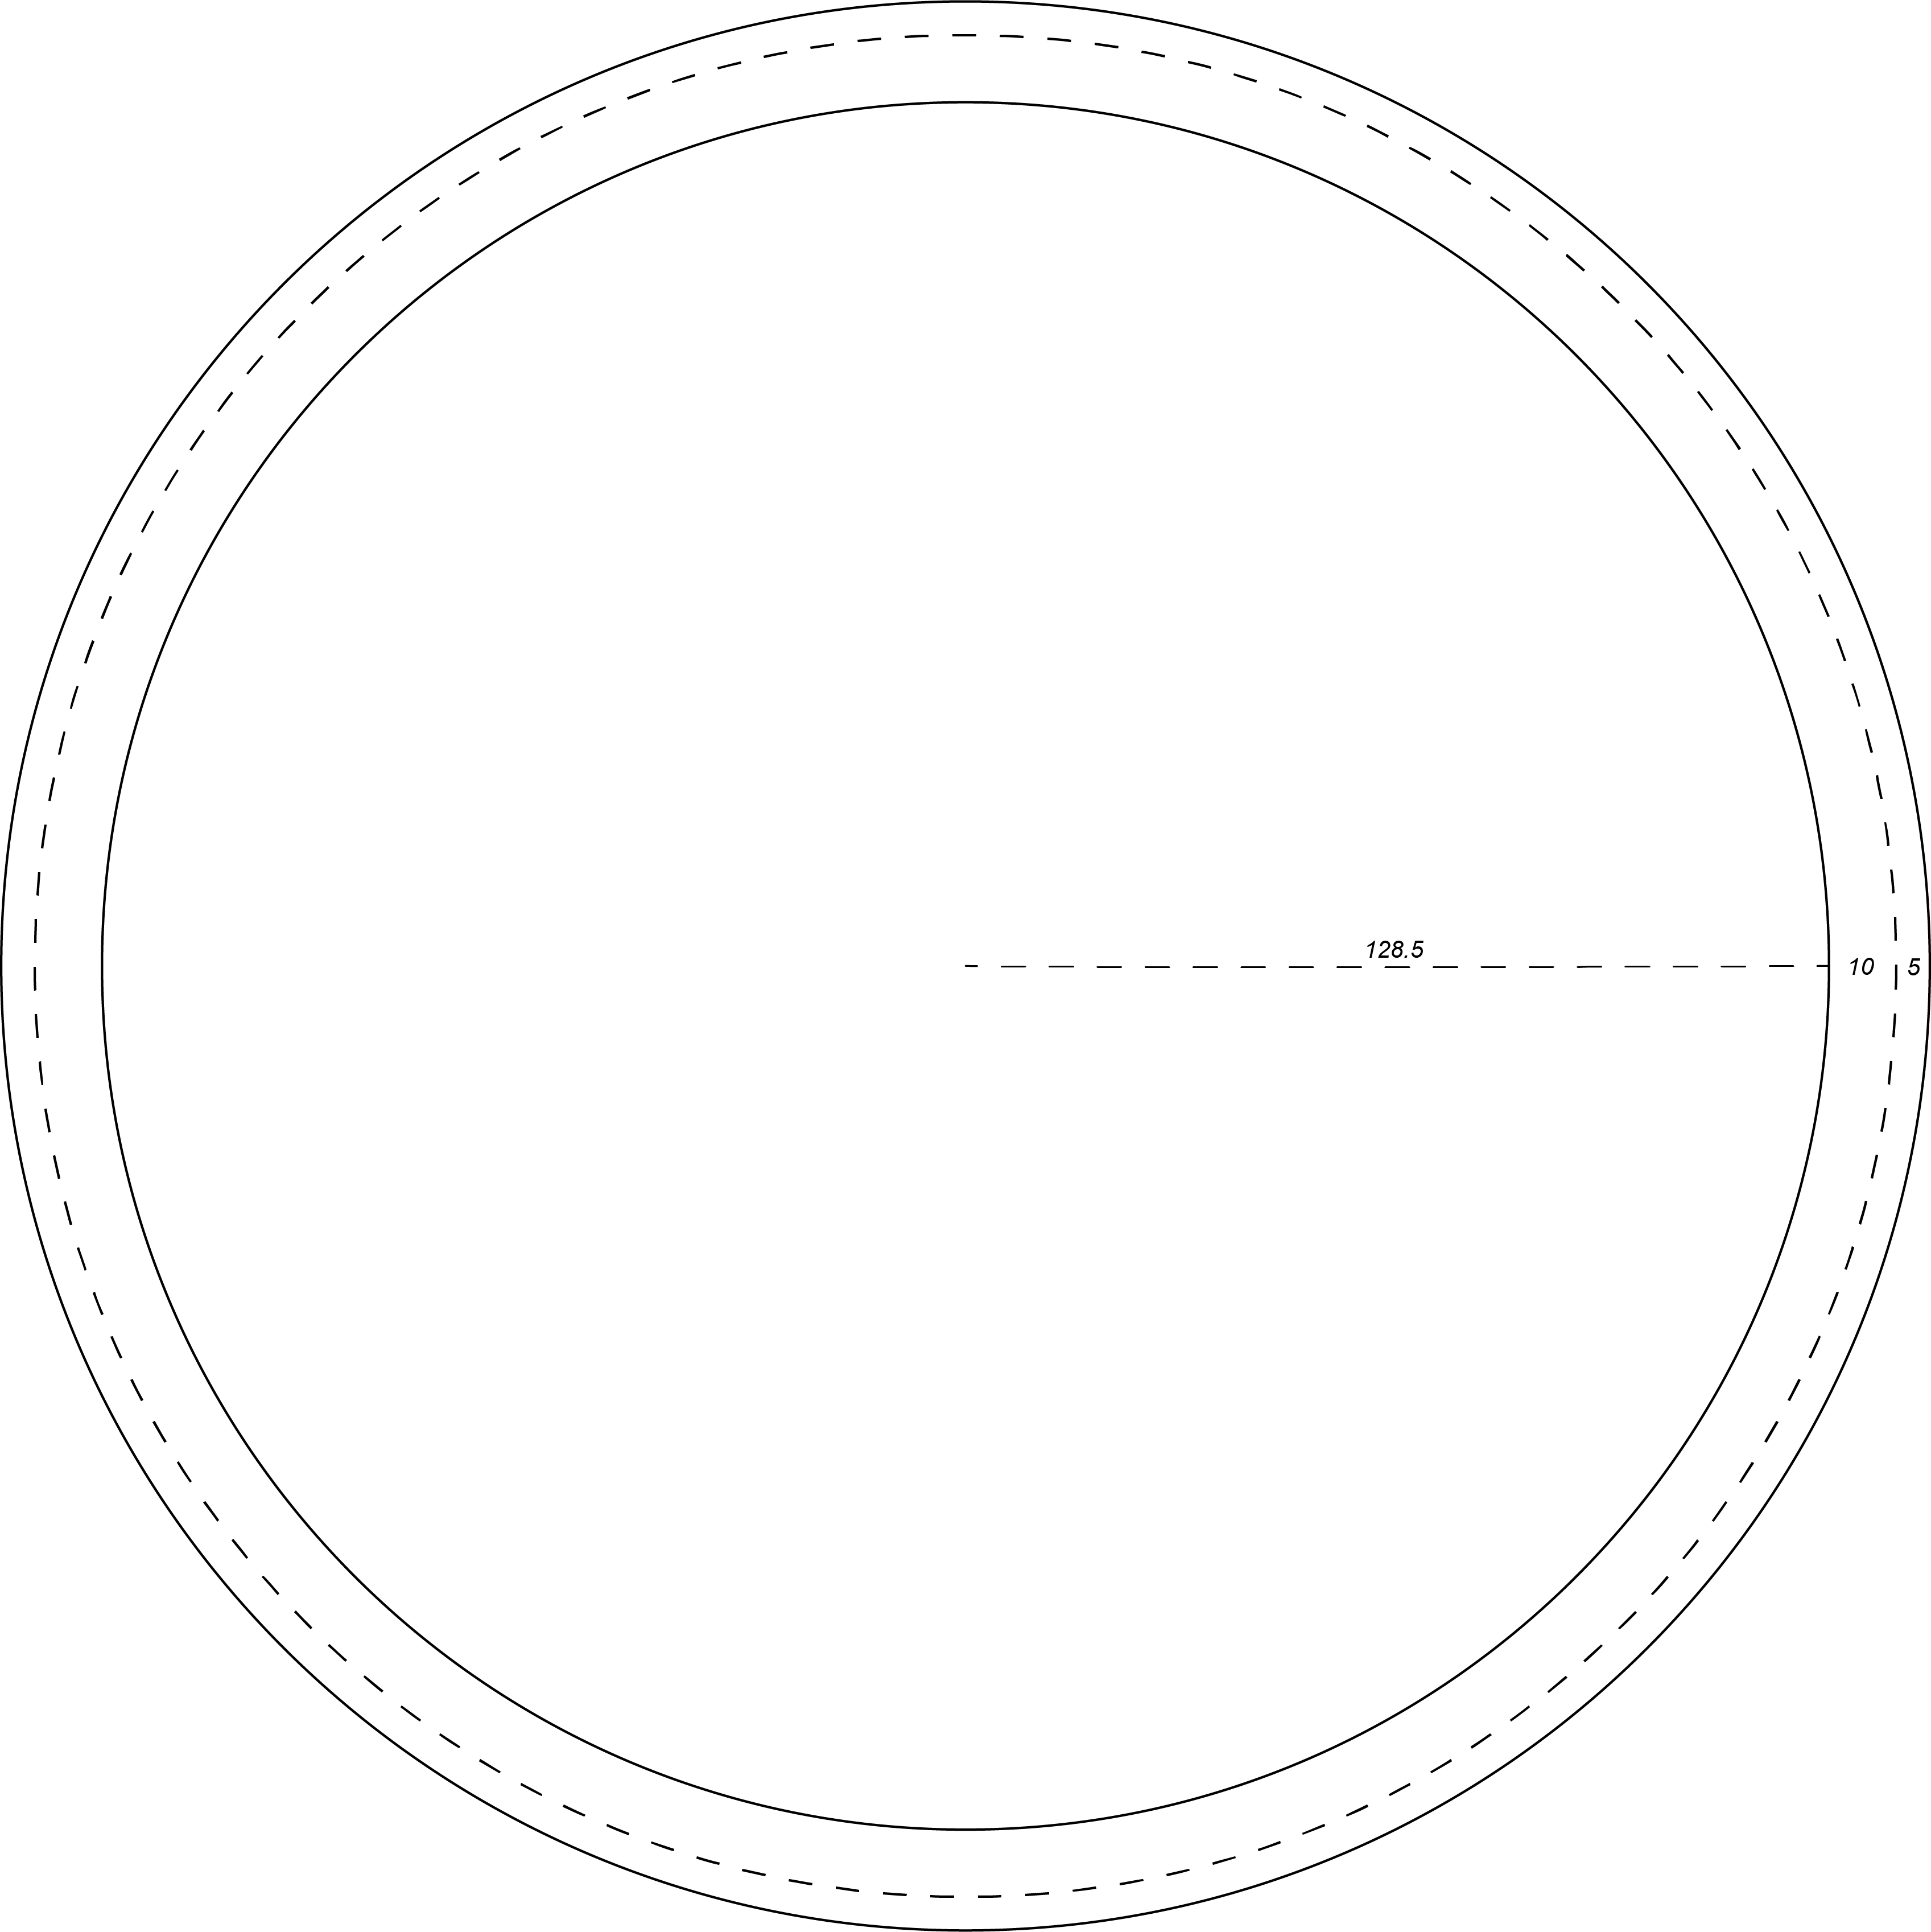
\includegraphics[width=0.5\textwidth]{vue de dessus plateau bas.jpg}
  \caption{Vue de dessus plateau bas}
\end{figure}
\begin{figure}[H]
  \centering
  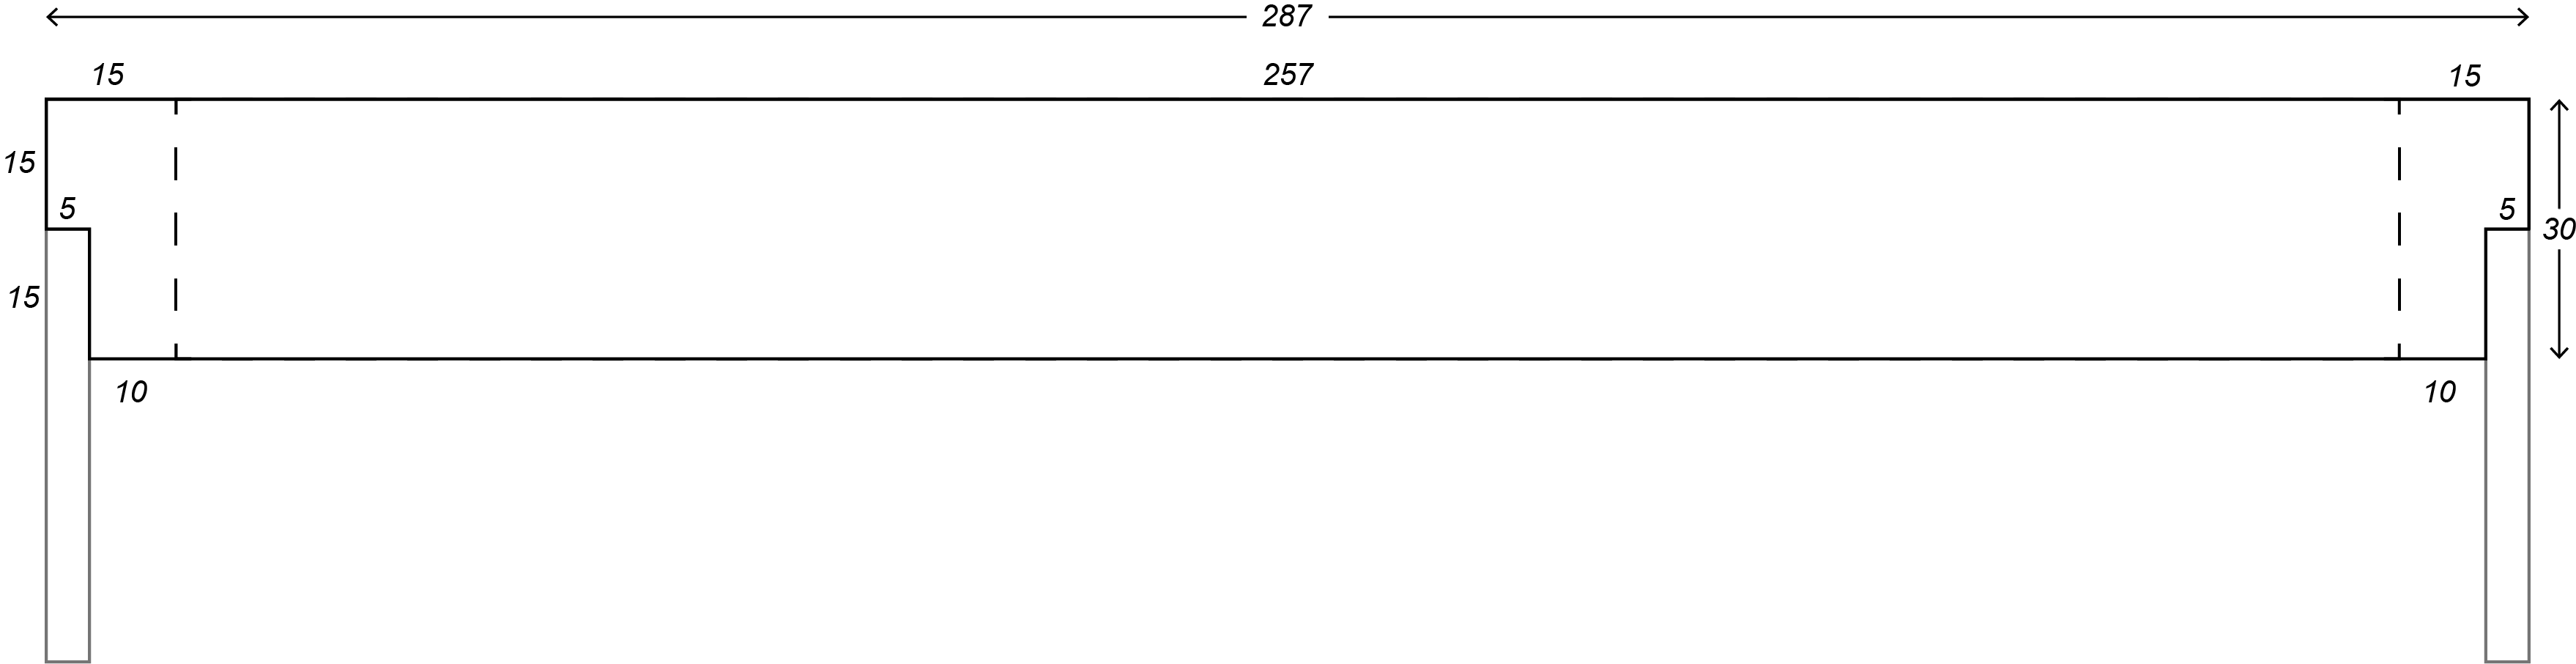
\includegraphics[width=0.5\textwidth]{vue de coupe plateau bas.jpg}
  \caption{Vue de coupe plateau bas}
\end{figure}

\subsubsubsection{Plateau supérieur}

Pour le plateau supérieur, la première contrainte est la même : obstruer le moins possible le passage de la lumière.
Mais sachant que ce plateau doit porter en son centre une caméra, la tâche est plus compliquée que précédemment ; nous y reviendrons point par point.
Comme le plateau doit porter une caméra, il doit être en conséquence assez résistant, donc plus large.
Nous ne modélisons donc, sur le même principe que le plateau inférieur, que les bords extérieurs et laissons le centre évidé pour laisser passer la lumière.  
Il doit aussi contenir de la matière au centre  pour poser la caméra. Nous modélisons donc un rond central évidé où emboîter la caméra. 
La question d’obstruction de la lumière ne vient pas ici car la caméra étant posée dessus, elle obstruerait de toute façon la lumière.
Il nous faut maintenant relier le cercle central aux bordures car seulement les bordures seront portées par les tendeurs, nous le rappelons. 
Il faut modéliser des branches reliant les différentes parties du plateau. Mais pas trop en nombre ni trop larges pour ne pas obstruer la lumière. 
Nous modélisons donc trois branches, nombre raisonnable choisi arbitrairement, mais facilitant la modélisation par rapport aux six trous sur le plateau qui seront groupés par deux. 
Pour augmenter la résistance des branches sans obstruer davantage la lumière, nous les modélisons avec plus de matière dans le sens de la hauteur.
Mais si toute la plateforme est faite ainsi, il y aura un problème pour l’accès des tendeurs entre les deux plateformes avec le surplus de matière les empêchant de bouger sans contrainte. 
Nous enlevons donc de la matière petit à petit à partir du centre, laissant ainsi une partie volumineuse et solide au niveau de la caméra et une partie plus fine en extérieur laissant plus libre champ aux tendeurs.

\begin{figure}[H]
  \centering
  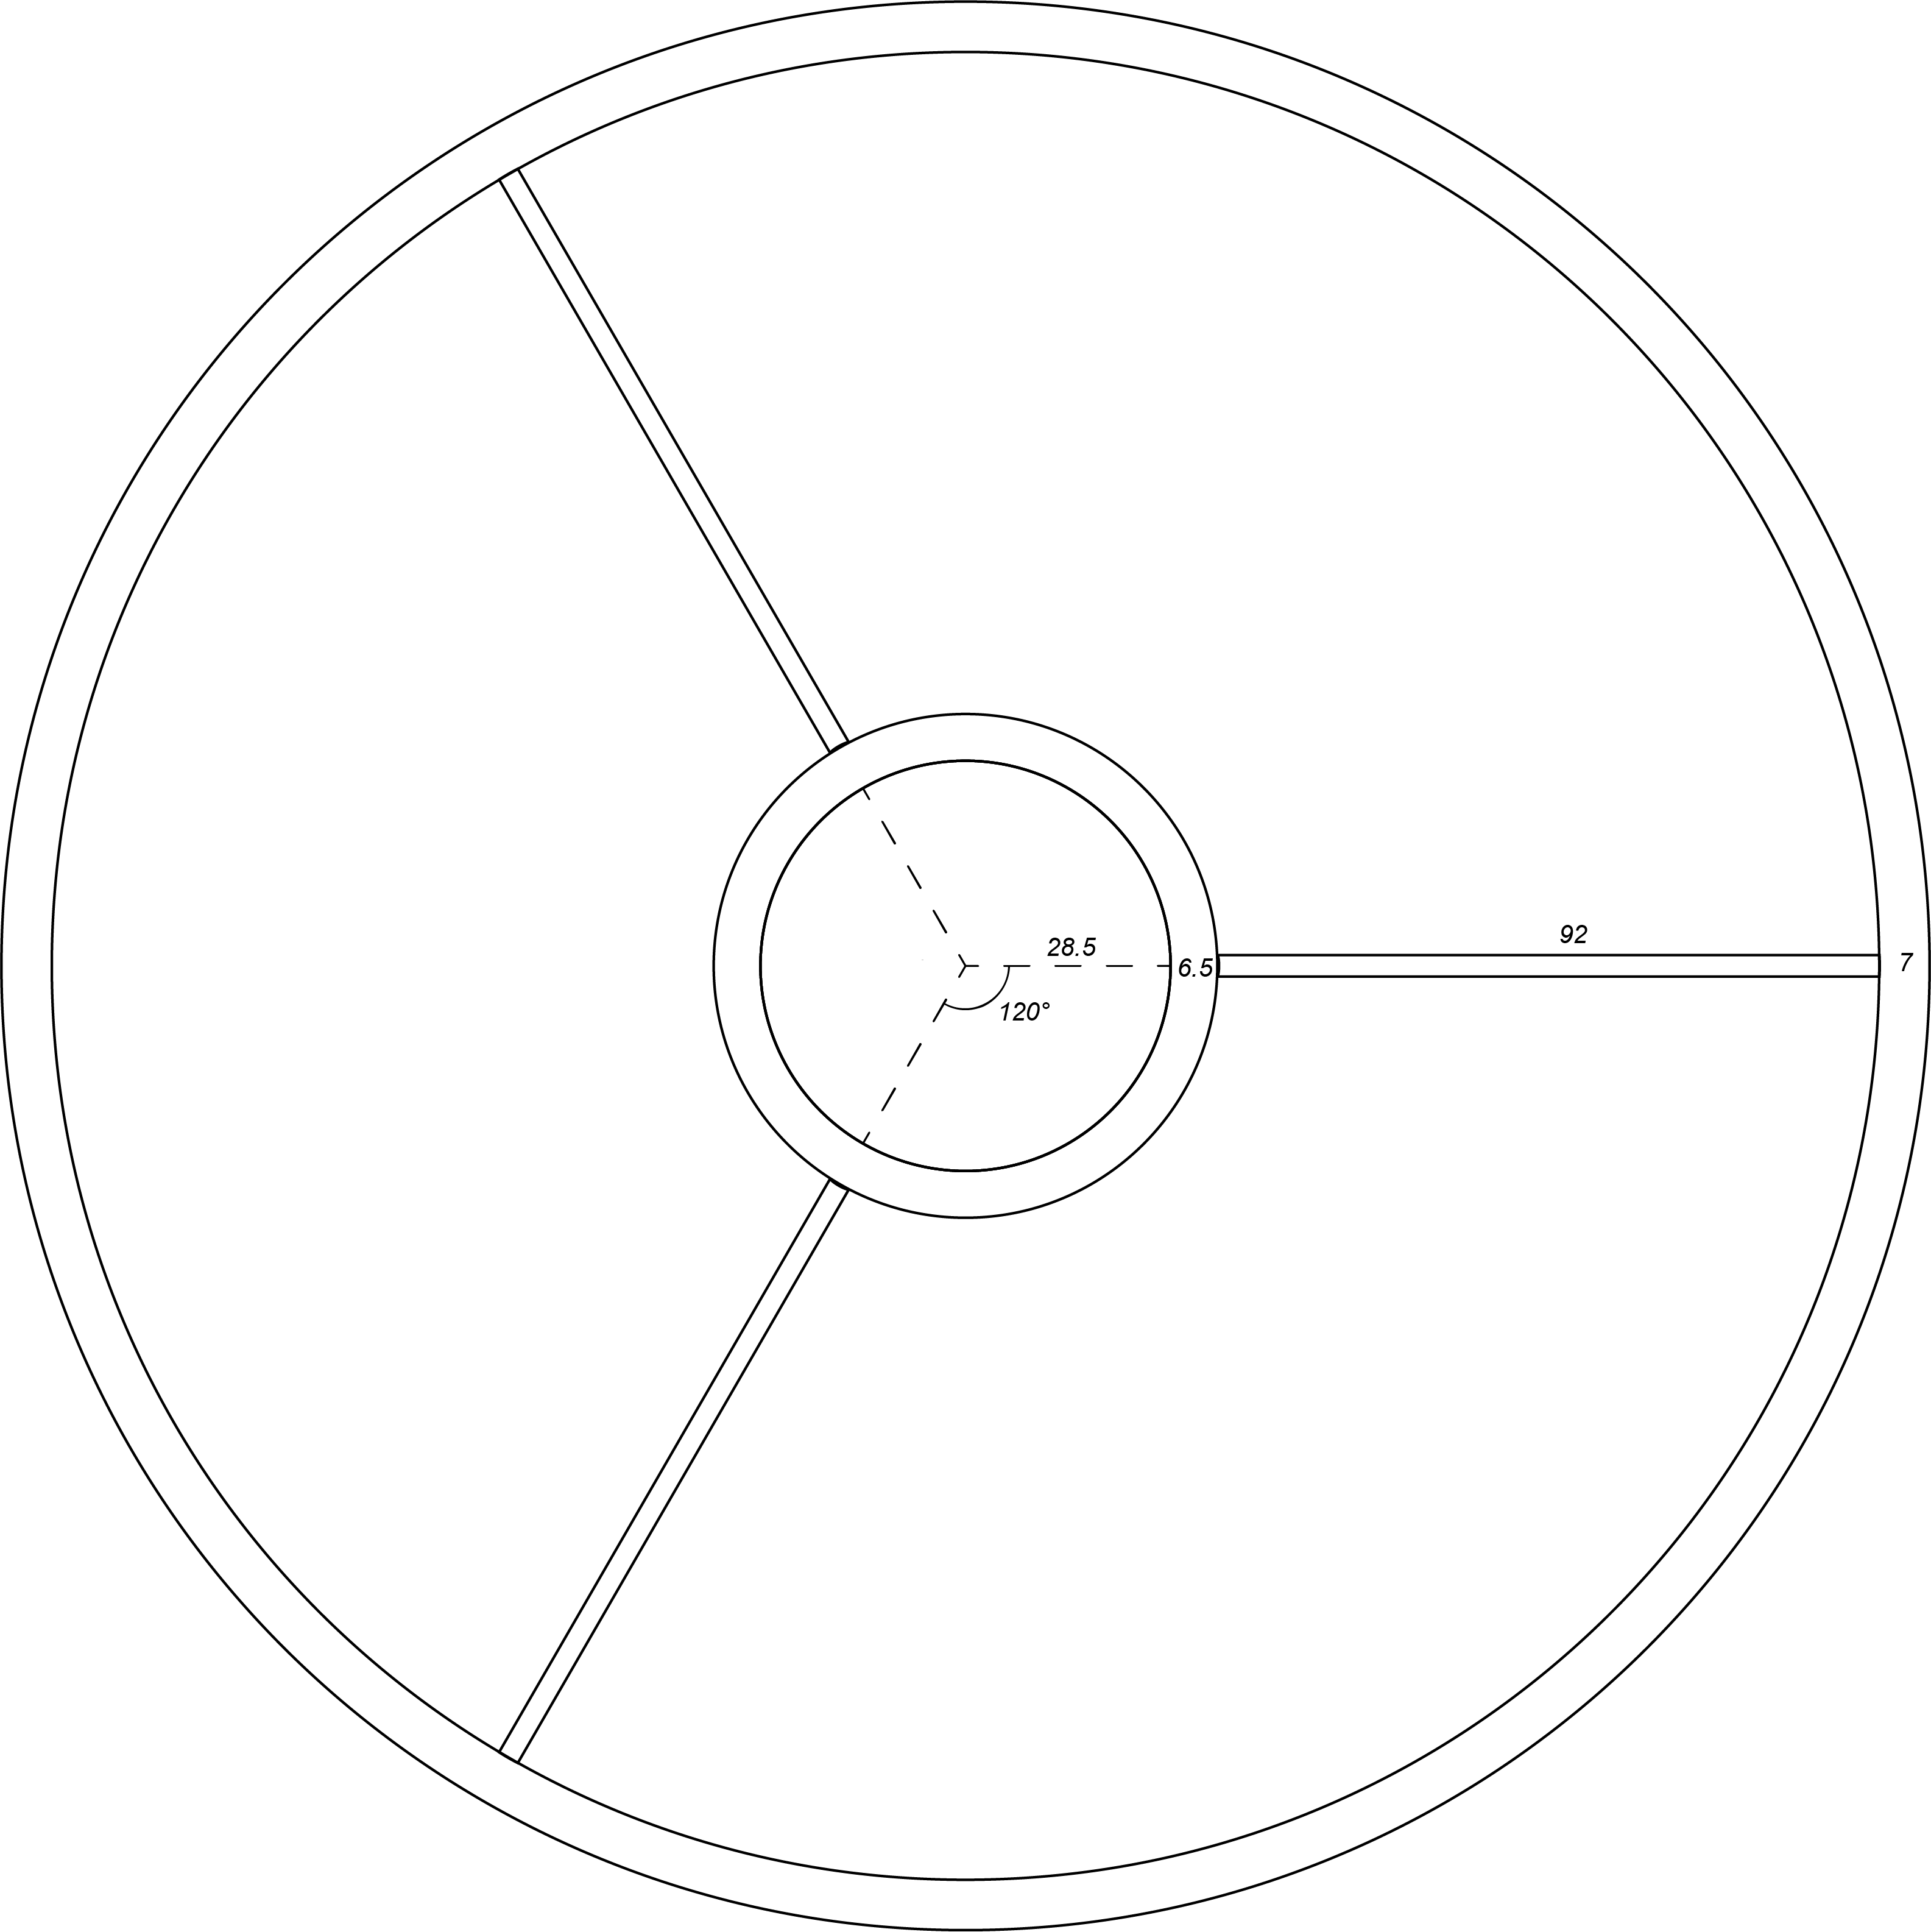
\includegraphics[width=0.6\textwidth]{vue de dessus plateau haut.jpg}
  \caption{Vue de dessus plateau haut}
\end{figure}

\begin{figure}[H]
  \centering
  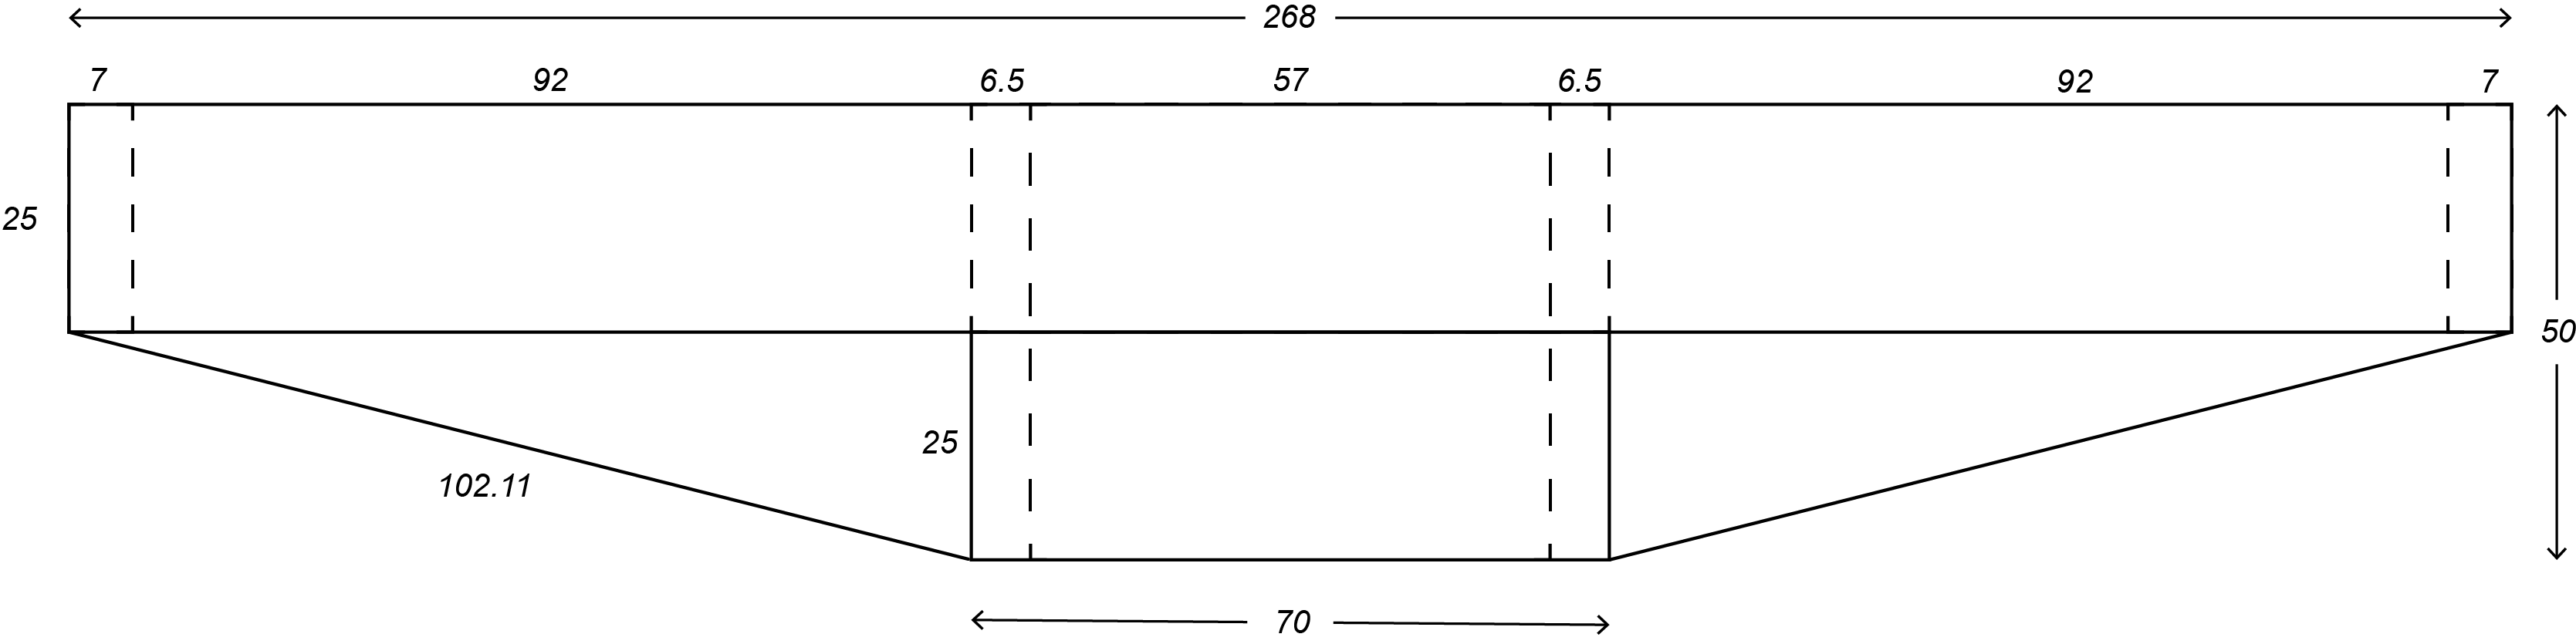
\includegraphics[width=0.7\textwidth]{vue de coupe plateau haut.jpg}
  \caption{Vue de coupe plateau haut}
\end{figure}

\subsubsection{Modélisation de la plateforme}

\subsubsubsection{Plateau inférieur}

Modélisation du plateau inférieur :
modélisation avec le logiciel FreeCAD. Fonctionnement à partir de schéma 2D auquel nous rajoutons de la matière. Nous réalisons donc d’abord sur le schéma deux cercles différents avec les diamètres  aux bordures afin d’y ajouter plus ou moins de matière et créer la bordure nécessaire.

\begin{figure}[H]
    \centering
    \begin{subfigure}[]{0.4\textwidth}
        \includegraphics[width=\textwidth]{mod plateau bas vide.png}
    \end{subfigure}
    \begin{subfigure}[]{0.4\textwidth}
        \includegraphics[width=\textwidth]{mod plateau bas plein.png}
    \end{subfigure}
    \caption{Schéma et modélisation du plateau bas}
\end{figure}

Pour finir, il nous faut modéliser des petits trous afin de faciliter le perçage après impression.
Pour enlever la matière, même principe que pour en créer : d’abord, faire un schéma 2D du trou recherché puis enlever la matière en fonction de ce schéma. 
Pour éviter de faire six schémas pour chacun des six trous, il existe une fonctionnalité sur FreeCAD qui répète une action de façon circulaire. Donc, une fois le premier trou modélisé, il suffit de rentrer le nombre de trous souhaités et ils sont repartis de façon régulière autour de l’axe choisi.

\begin{figure}[H]
    \centering
    \begin{subfigure}[]{0.4\textwidth}
        \includegraphics[width=\textwidth]{plan trou bas.png}
    \end{subfigure}
    \begin{subfigure}[]{0.4\textwidth}
        \includegraphics[width=\textwidth]{plat bas 6 trous.png}
    \end{subfigure}
    \caption{Schéma et modélisation des trous du plateau bas}
\end{figure}

\subsubsubsection{Plateau supérieur}

Même principe pour le plateau supérieur. D’abord, effectuer le schéma avant d’ajouter ou de retirer la matière.
Nous commençons donc par dessiner et modéliser juste une partie du plateau pour une question de précision lors du placement des branches. Puis, nous modélisons les trous au bout de la branche présente à l’aide toujours de schéma.

 
\begin{figure}[H]
    \centering
    \begin{subfigure}[]{0.25\textwidth}
        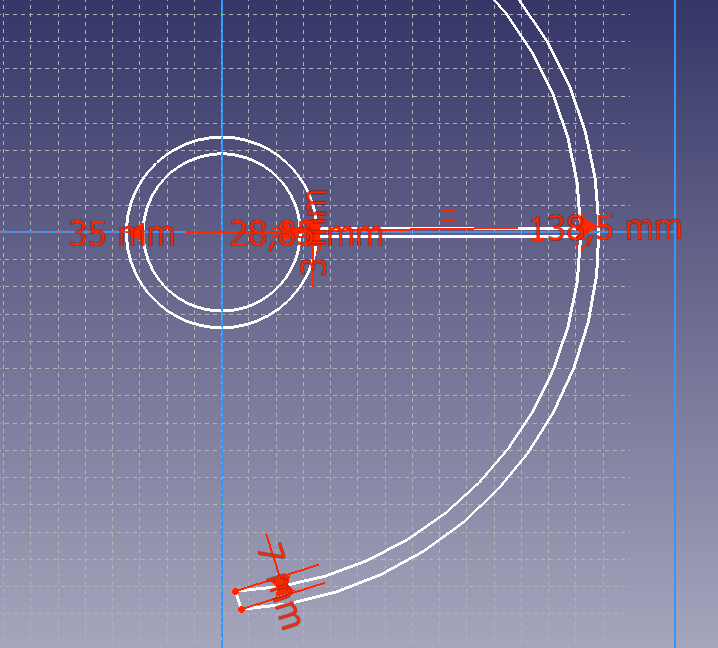
\includegraphics[width=\textwidth]{demi plat haut vide.png}
    \end{subfigure}
    \begin{subfigure}[]{0.3\textwidth}
        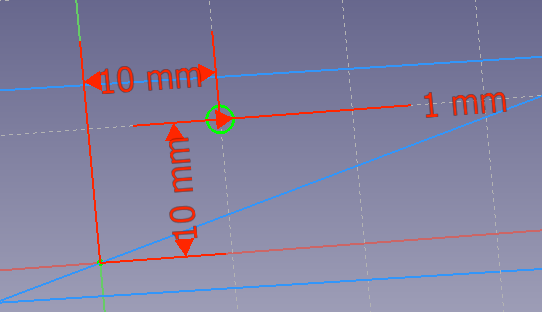
\includegraphics[width=\textwidth]{mod trou haut.png}
    \end{subfigure}
    \begin{subfigure}[]{0.3\textwidth}
        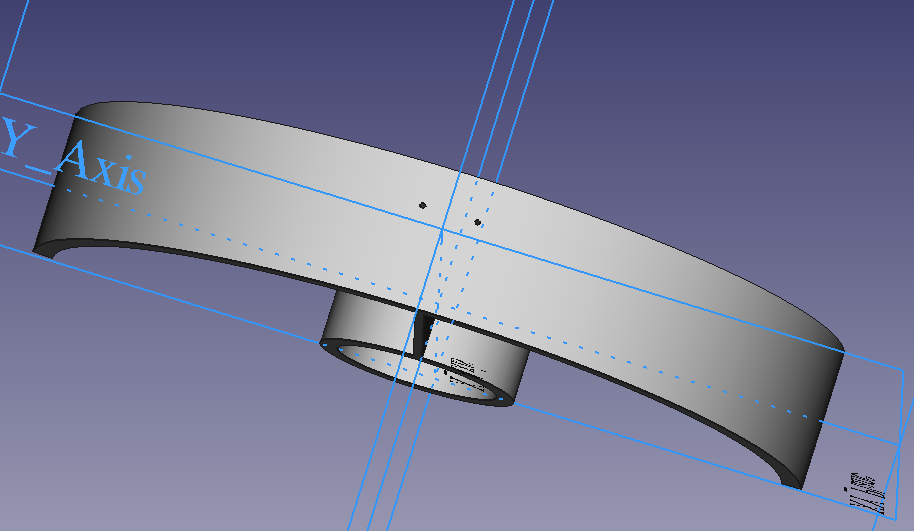
\includegraphics[width=\textwidth]{demi plat haut final.png}
    \end{subfigure}
    \caption{Schéma et modélisation du plateau et des trous du plateau haut}
\end{figure}

Puis, nous réutilisons la fonctionnalité de répétition circulaire pour refaire le tout trois fois afin d’avoir les trous et les branches à intervalles réguliers. Sur cette action, nous constatons que certaines parties de matière se chevauchent, mais cela n’est qu’un détail car lors de l’impression cela ne changera rien. 

\begin{figure}[H]
    \centering
    \includegraphics[width=0.6\textwidth]{plat haut trous.png}
    \caption{Plateau haut après l'utilisation de la fonctionnalité de répétition circulaire}
\end{figure}

Enfin, pour faciliter l’accès des tendeurs entre les deux plateaux, nous décidons de rogner de façon triangulaire les branches et l’anneau extérieur. Pour ce faire, toujours le même procédé : d’abord réaliser un schéma représentant la forme à rogner puis utiliser la fonctionnalité de déblaiement circulaire tout autour de l’axe central.

\begin{figure}[H]
    \centering
    \begin{subfigure}[]{0.4\textwidth}
        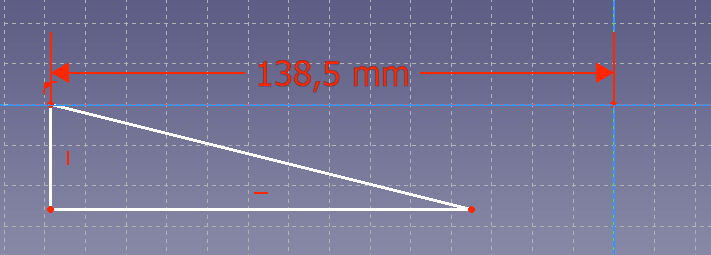
\includegraphics[width=\textwidth]{triangle.png}
    \end{subfigure}
    \begin{subfigure}[]{0.3\textwidth}
        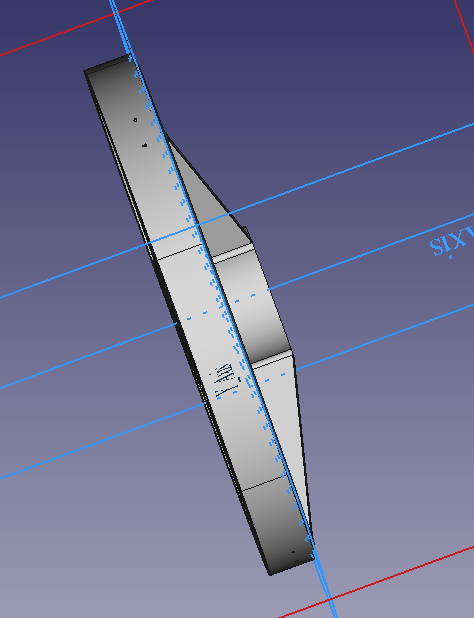
\includegraphics[width=\textwidth]{plat haut final.png}
    \end{subfigure}
    \caption{Schéma de la figure à rogner et plateau haut après rognage}
\end{figure}

\subsubsection{Impression de la plateforme}

Une fois toutes ces étapes réalisées, nous avons exporté les deux modélisations en fichier \og .stl \fg, fichier que l’imprimante est capable de lire. 
Puis, nous les avons mis sur clé et les avons connectés à l’imprimante pour impression.



\newpage

\section{Expérimentation}

Une fois les pièces imprimées et les bielles reçues, nous sommes passés à la construction de la plateforme. 
Là, un problème est apparu dès le démarrage. 
Les trous du plateau bas sont trop espacés pour qu'il y ait un espace suffisant entre les deux plateaux. 
Pour satisfaire à la résolution de ce problème, nous décidons de réduire l'espace entre ceux-ci à quatre-vingt-quinze millimètres -c'est la distance trou à trou en ligne droite-, cela nous permettant d'obtenir une hauteur entre les deux plateaux de cinquante millimètres. 
Nous perçons des trous de trois millimètres de diamètre pour y insérer vis et écrous et ainsi assurer une bonne fixation. De plus, nous plaçons des rondelles de part et d'autre des rotules afin que celles-ci puissent avoir un mouvement libre et nous plaçons également des rondelles avant les écrous pour éviter que cela n’endommage les plateaux qui sont en acide polylactique (PLA), une matière plastique d’origine végétale, utilisée en impression 3D. 

\begin{figure}[H]
  \centering
  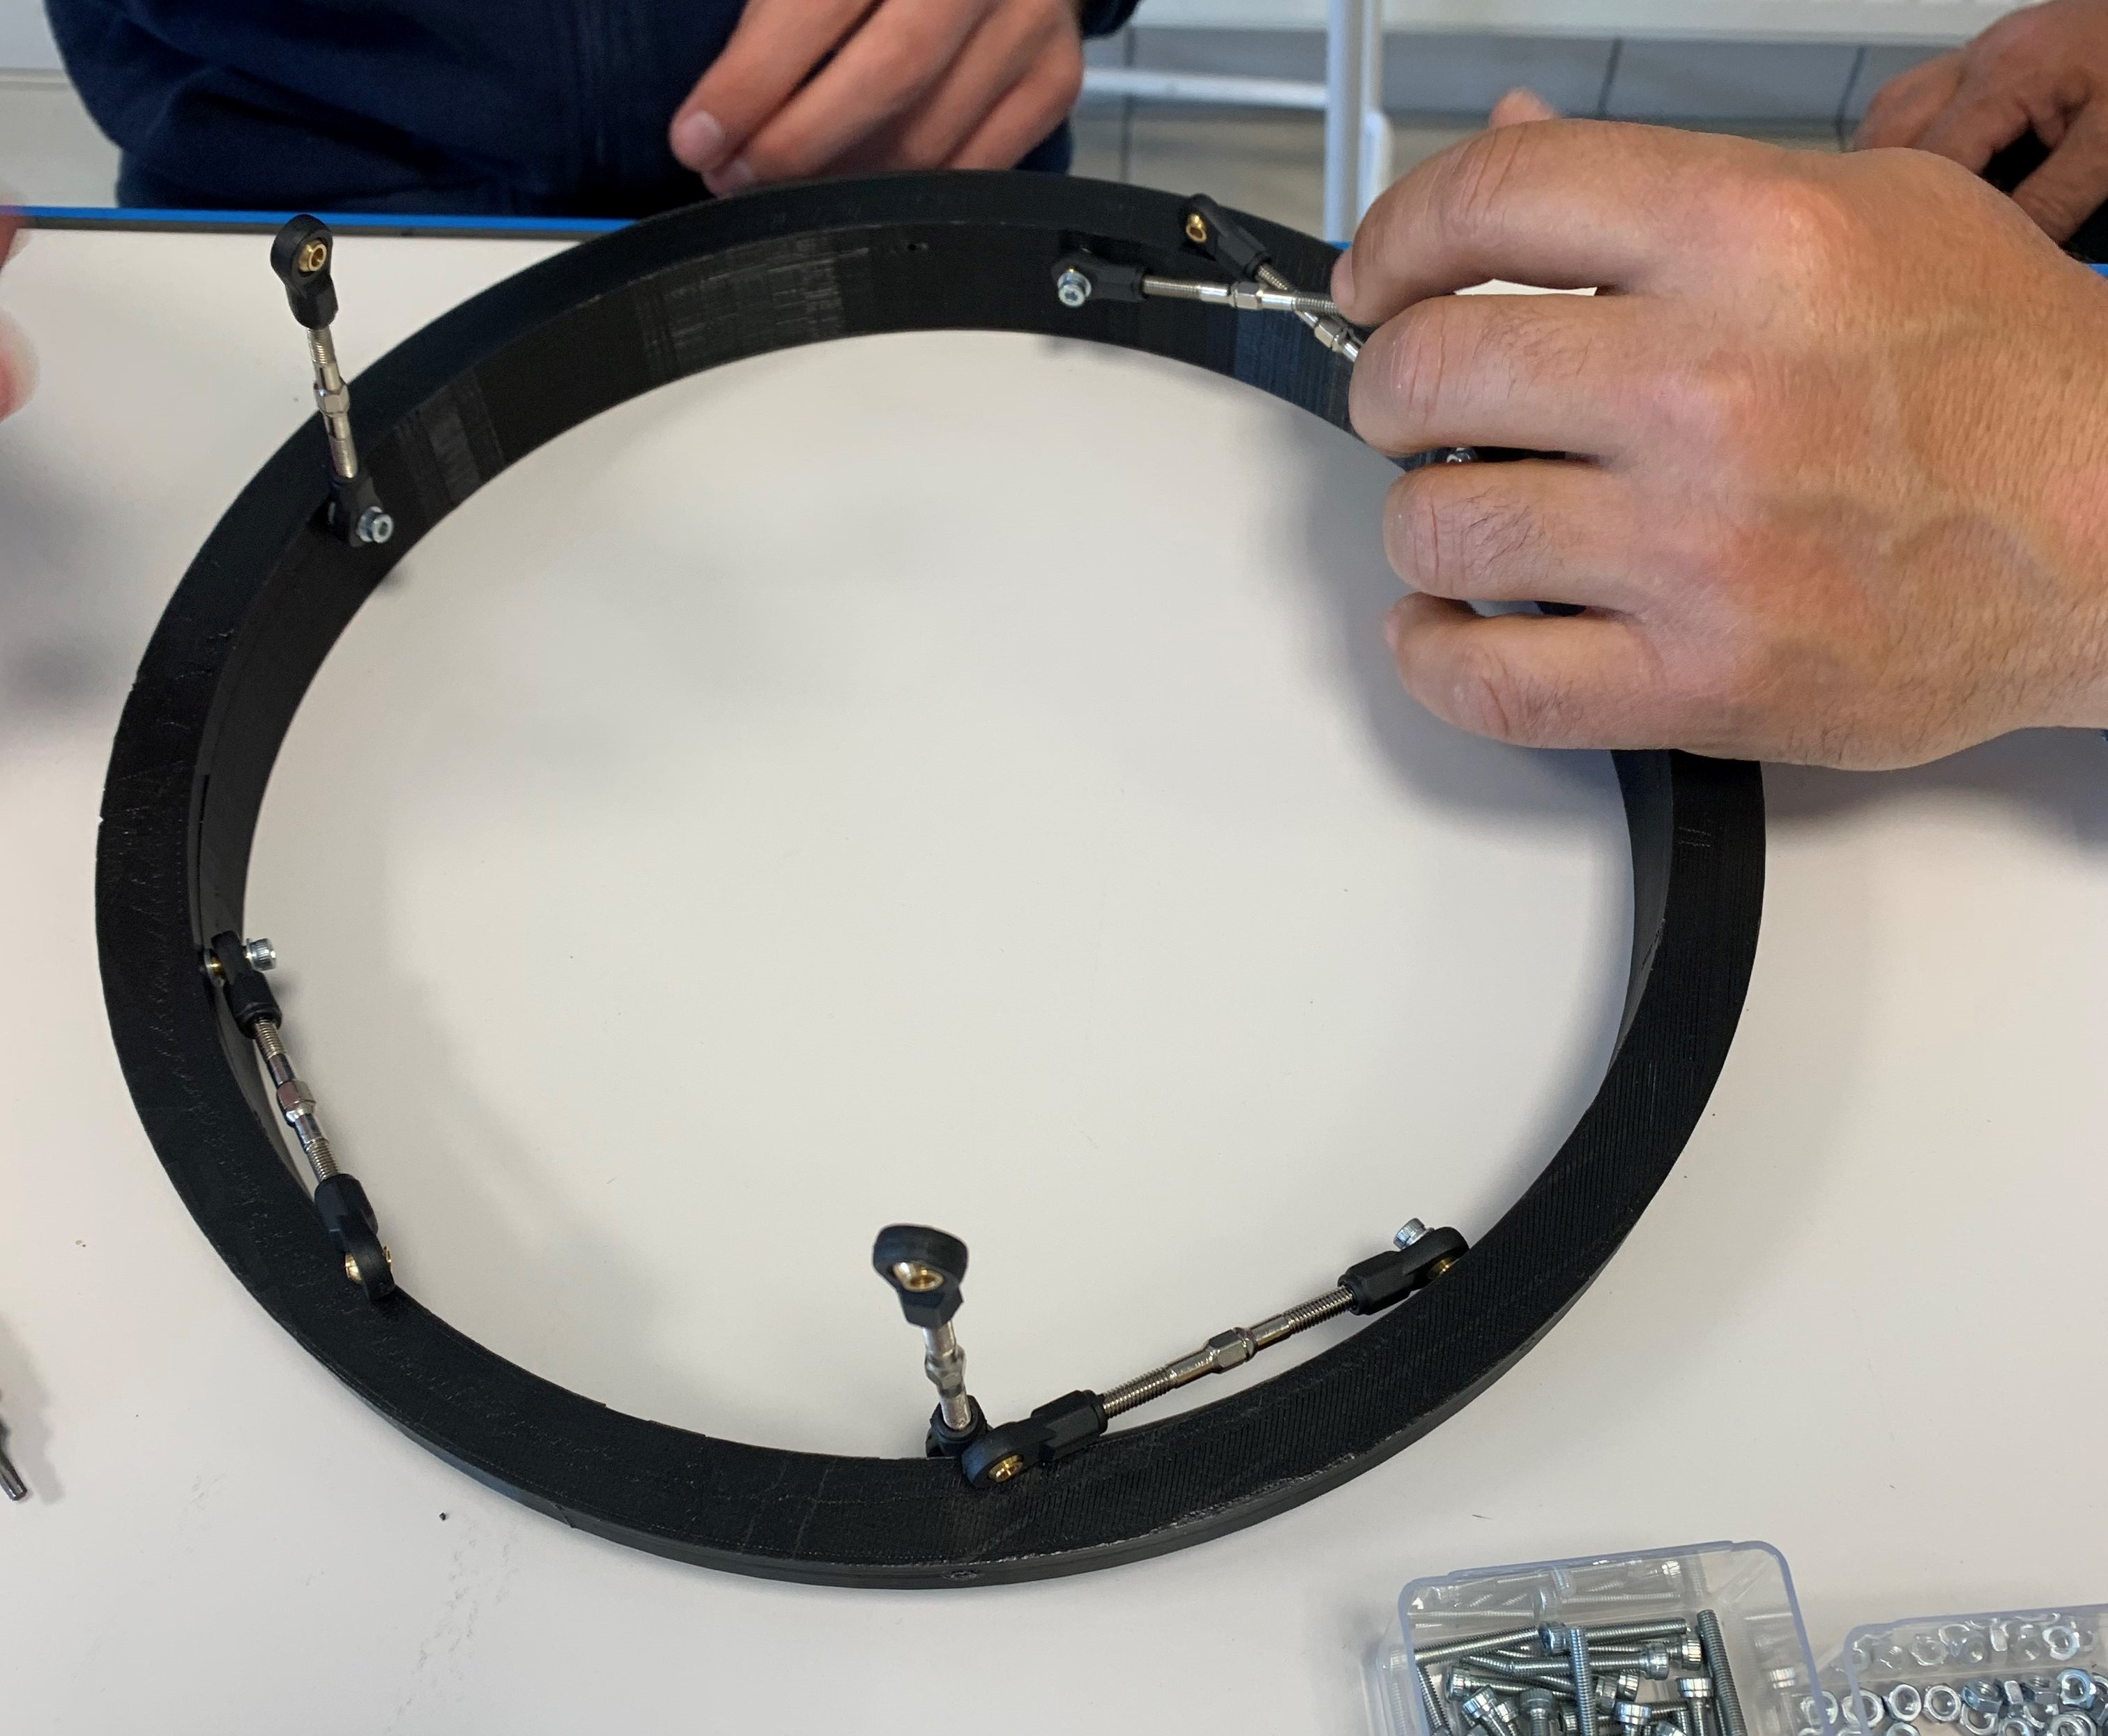
\includegraphics[width=0.6\textwidth]{montage plateforme.jpg}
  \caption{Montage de la plateforme}
\end{figure}

La deuxième étape consiste à mettre la plateforme à niveau.
Cependant, un problème est apparu ici. En effet, il y a une translation horizontale qui s'est créée entre les deux plateaux. Leurs centres ne sont plus alignés par une droite normale au plateau bas.
Ce problème vient du fait que, lors de l'impression, nous avions paramétré un espacement régulier des trous de fixations.
Toutefois, pour s'adapter aux contraintes venant des bielles, nous modifions l'espacement de ceux-ci  pour pouvoir réaliser le montage de la plateforme. 
En perçant donc de nouveaux trous dans le plateau bas pour remédier au problème de longueur des bielles, nous commettons des erreurs expérimentales et cela crée une sorte de déséquilibre de la plateforme. Les deux centres des plateaux ne sont donc plus parfaitement alignés, cependant nous réussissons à ce que les plateaux soient parallèles, ce qui est très important pour le fonctionnement sur le télescope. 
En effet, si les deux plateaux ne sont pas parallèles, il est impossible de prendre un cliché net avec la caméra placée sur le plateau haut. 
Cette translation montre aussi un autre aspect positif du montage, celui du déplacement du plateau qui se contrôle grâce à la longueur des bielles. 
En observant les longueurs des six bielles, nous remarquons que la position parallèle obtenue ne vient pas du fait que celles-ci sont les mêmes. C'est ce que nous avions fait au début. Nous avions monté la plateforme en mettant les six bielles à la même longueur et cela créait une inclinaison du plateau haut par rapport au plateau bas. 



\begin{figure}[H]
    \centering
    \begin{subfigure}[]{0.4\textwidth}
        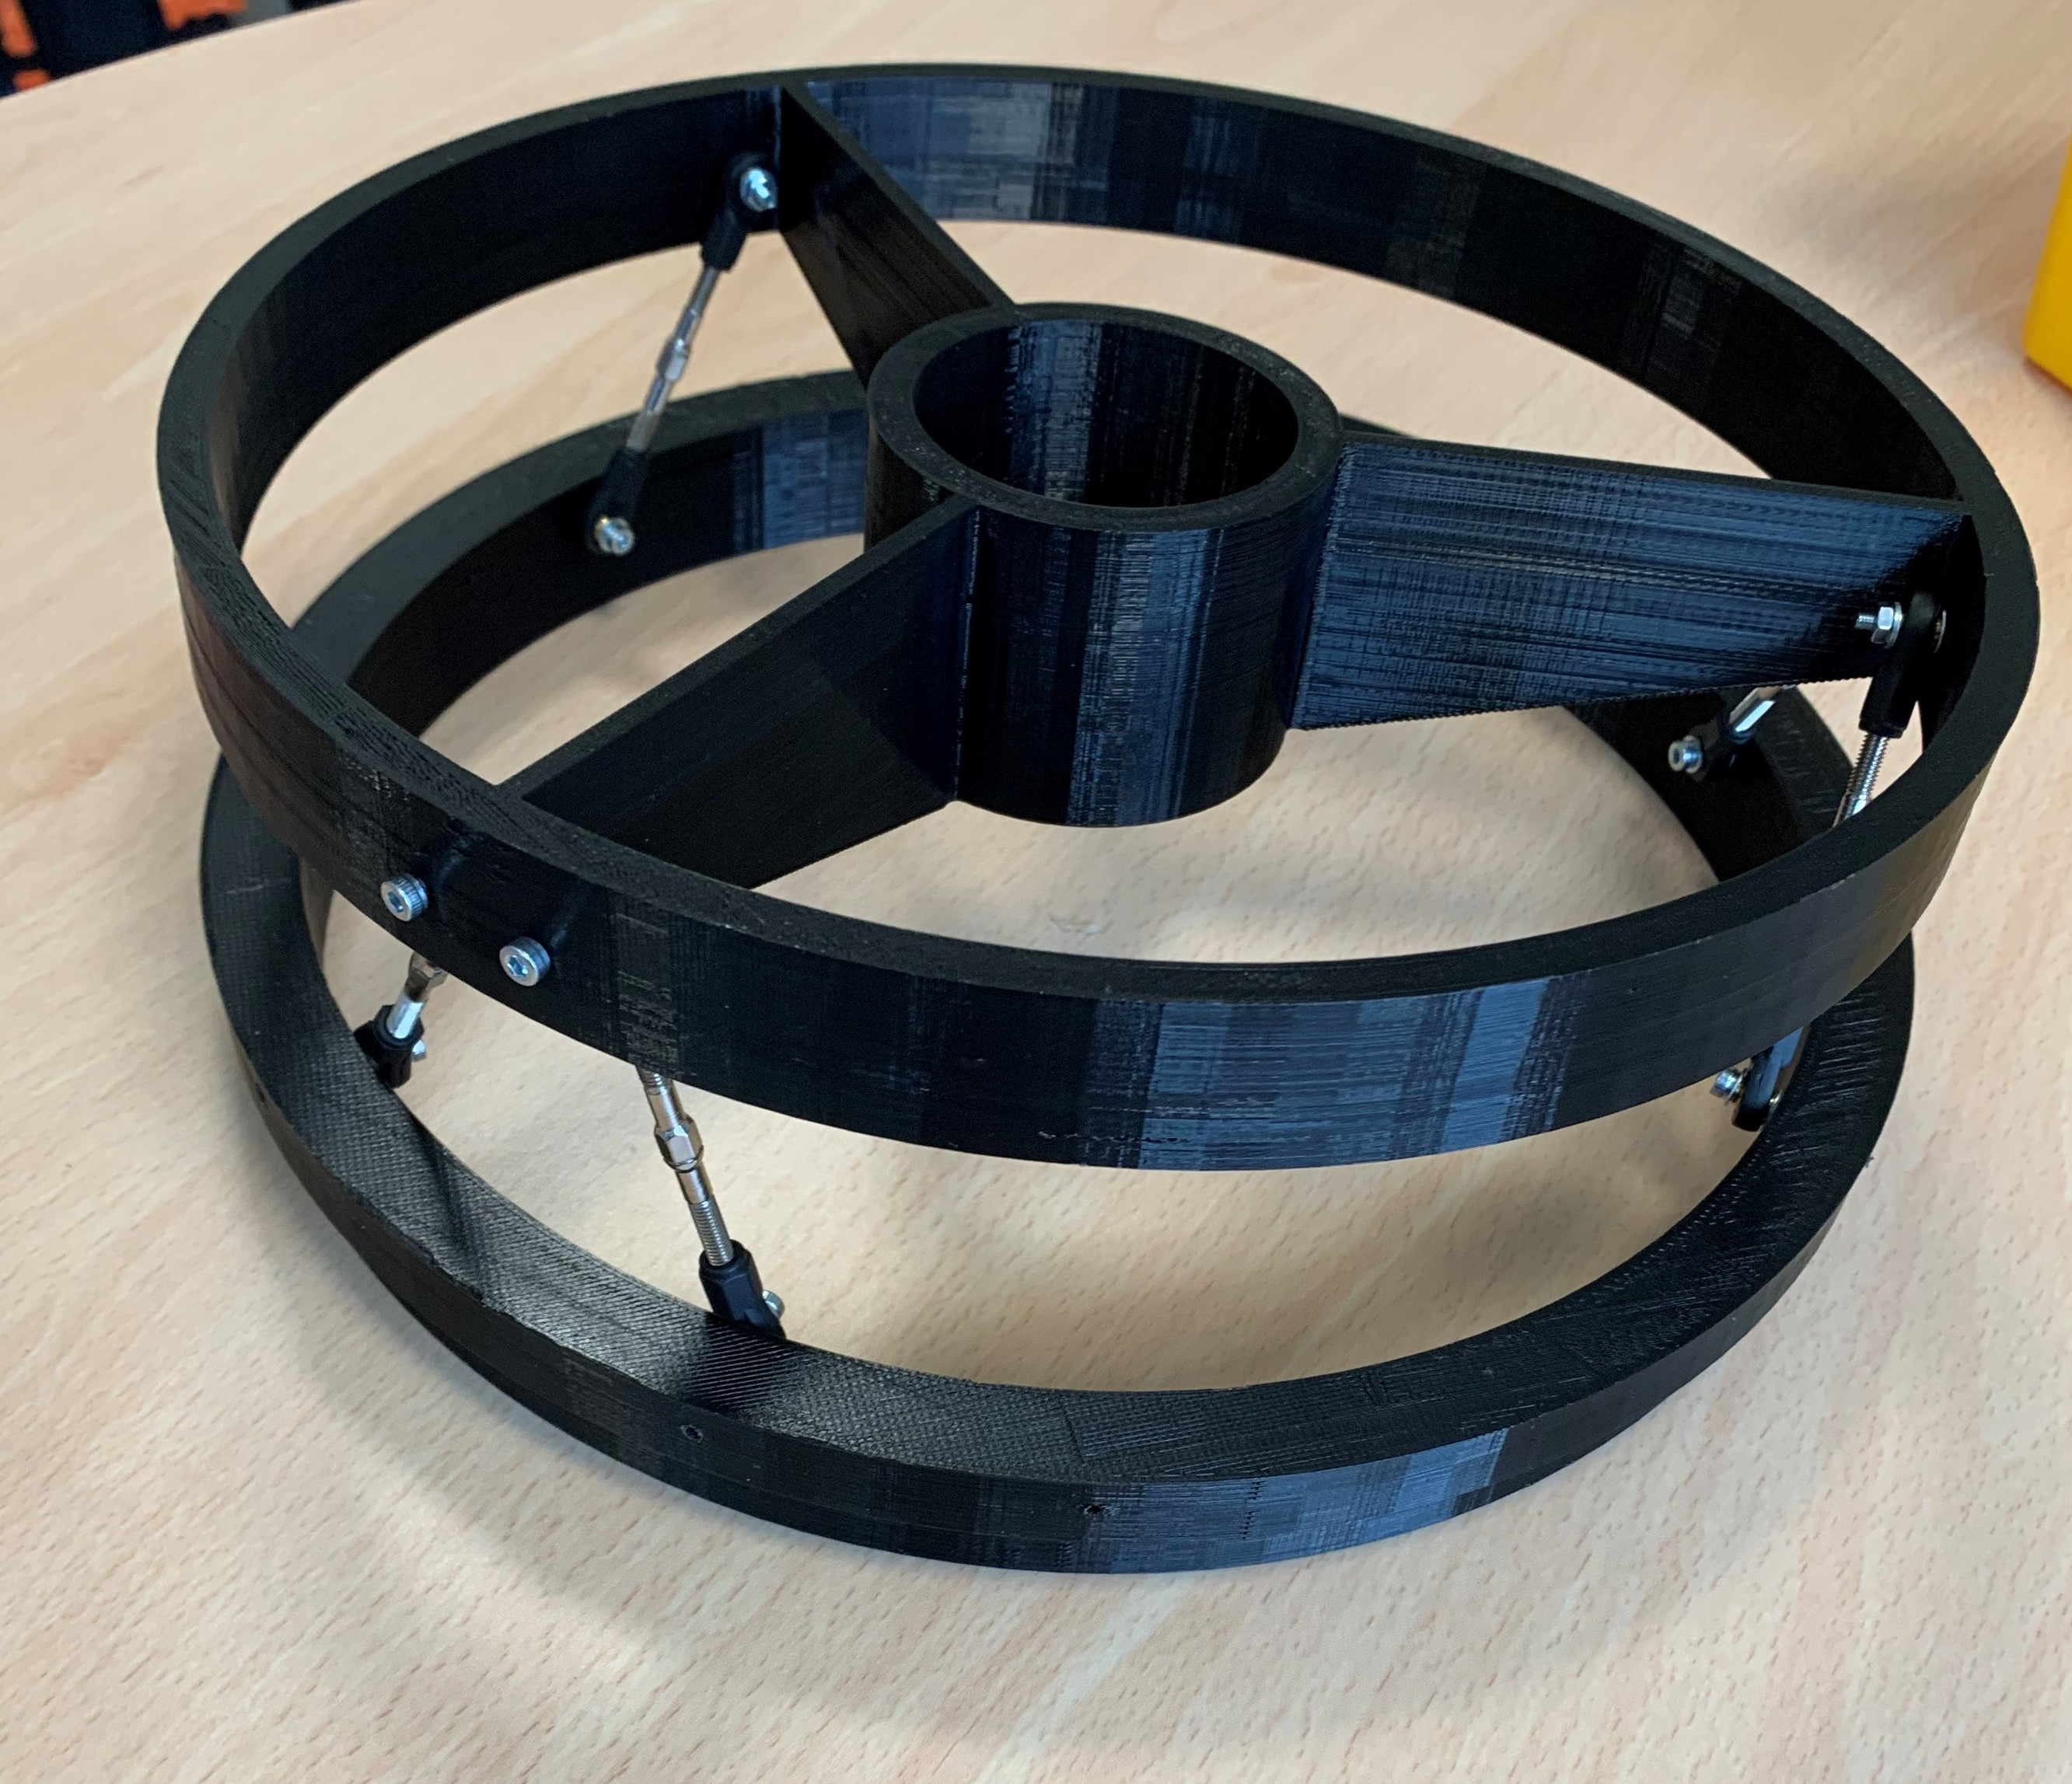
\includegraphics[width=\textwidth]{plateforme 1.jpg}
    \end{subfigure}
    \begin{subfigure}[]{0.5\textwidth}
        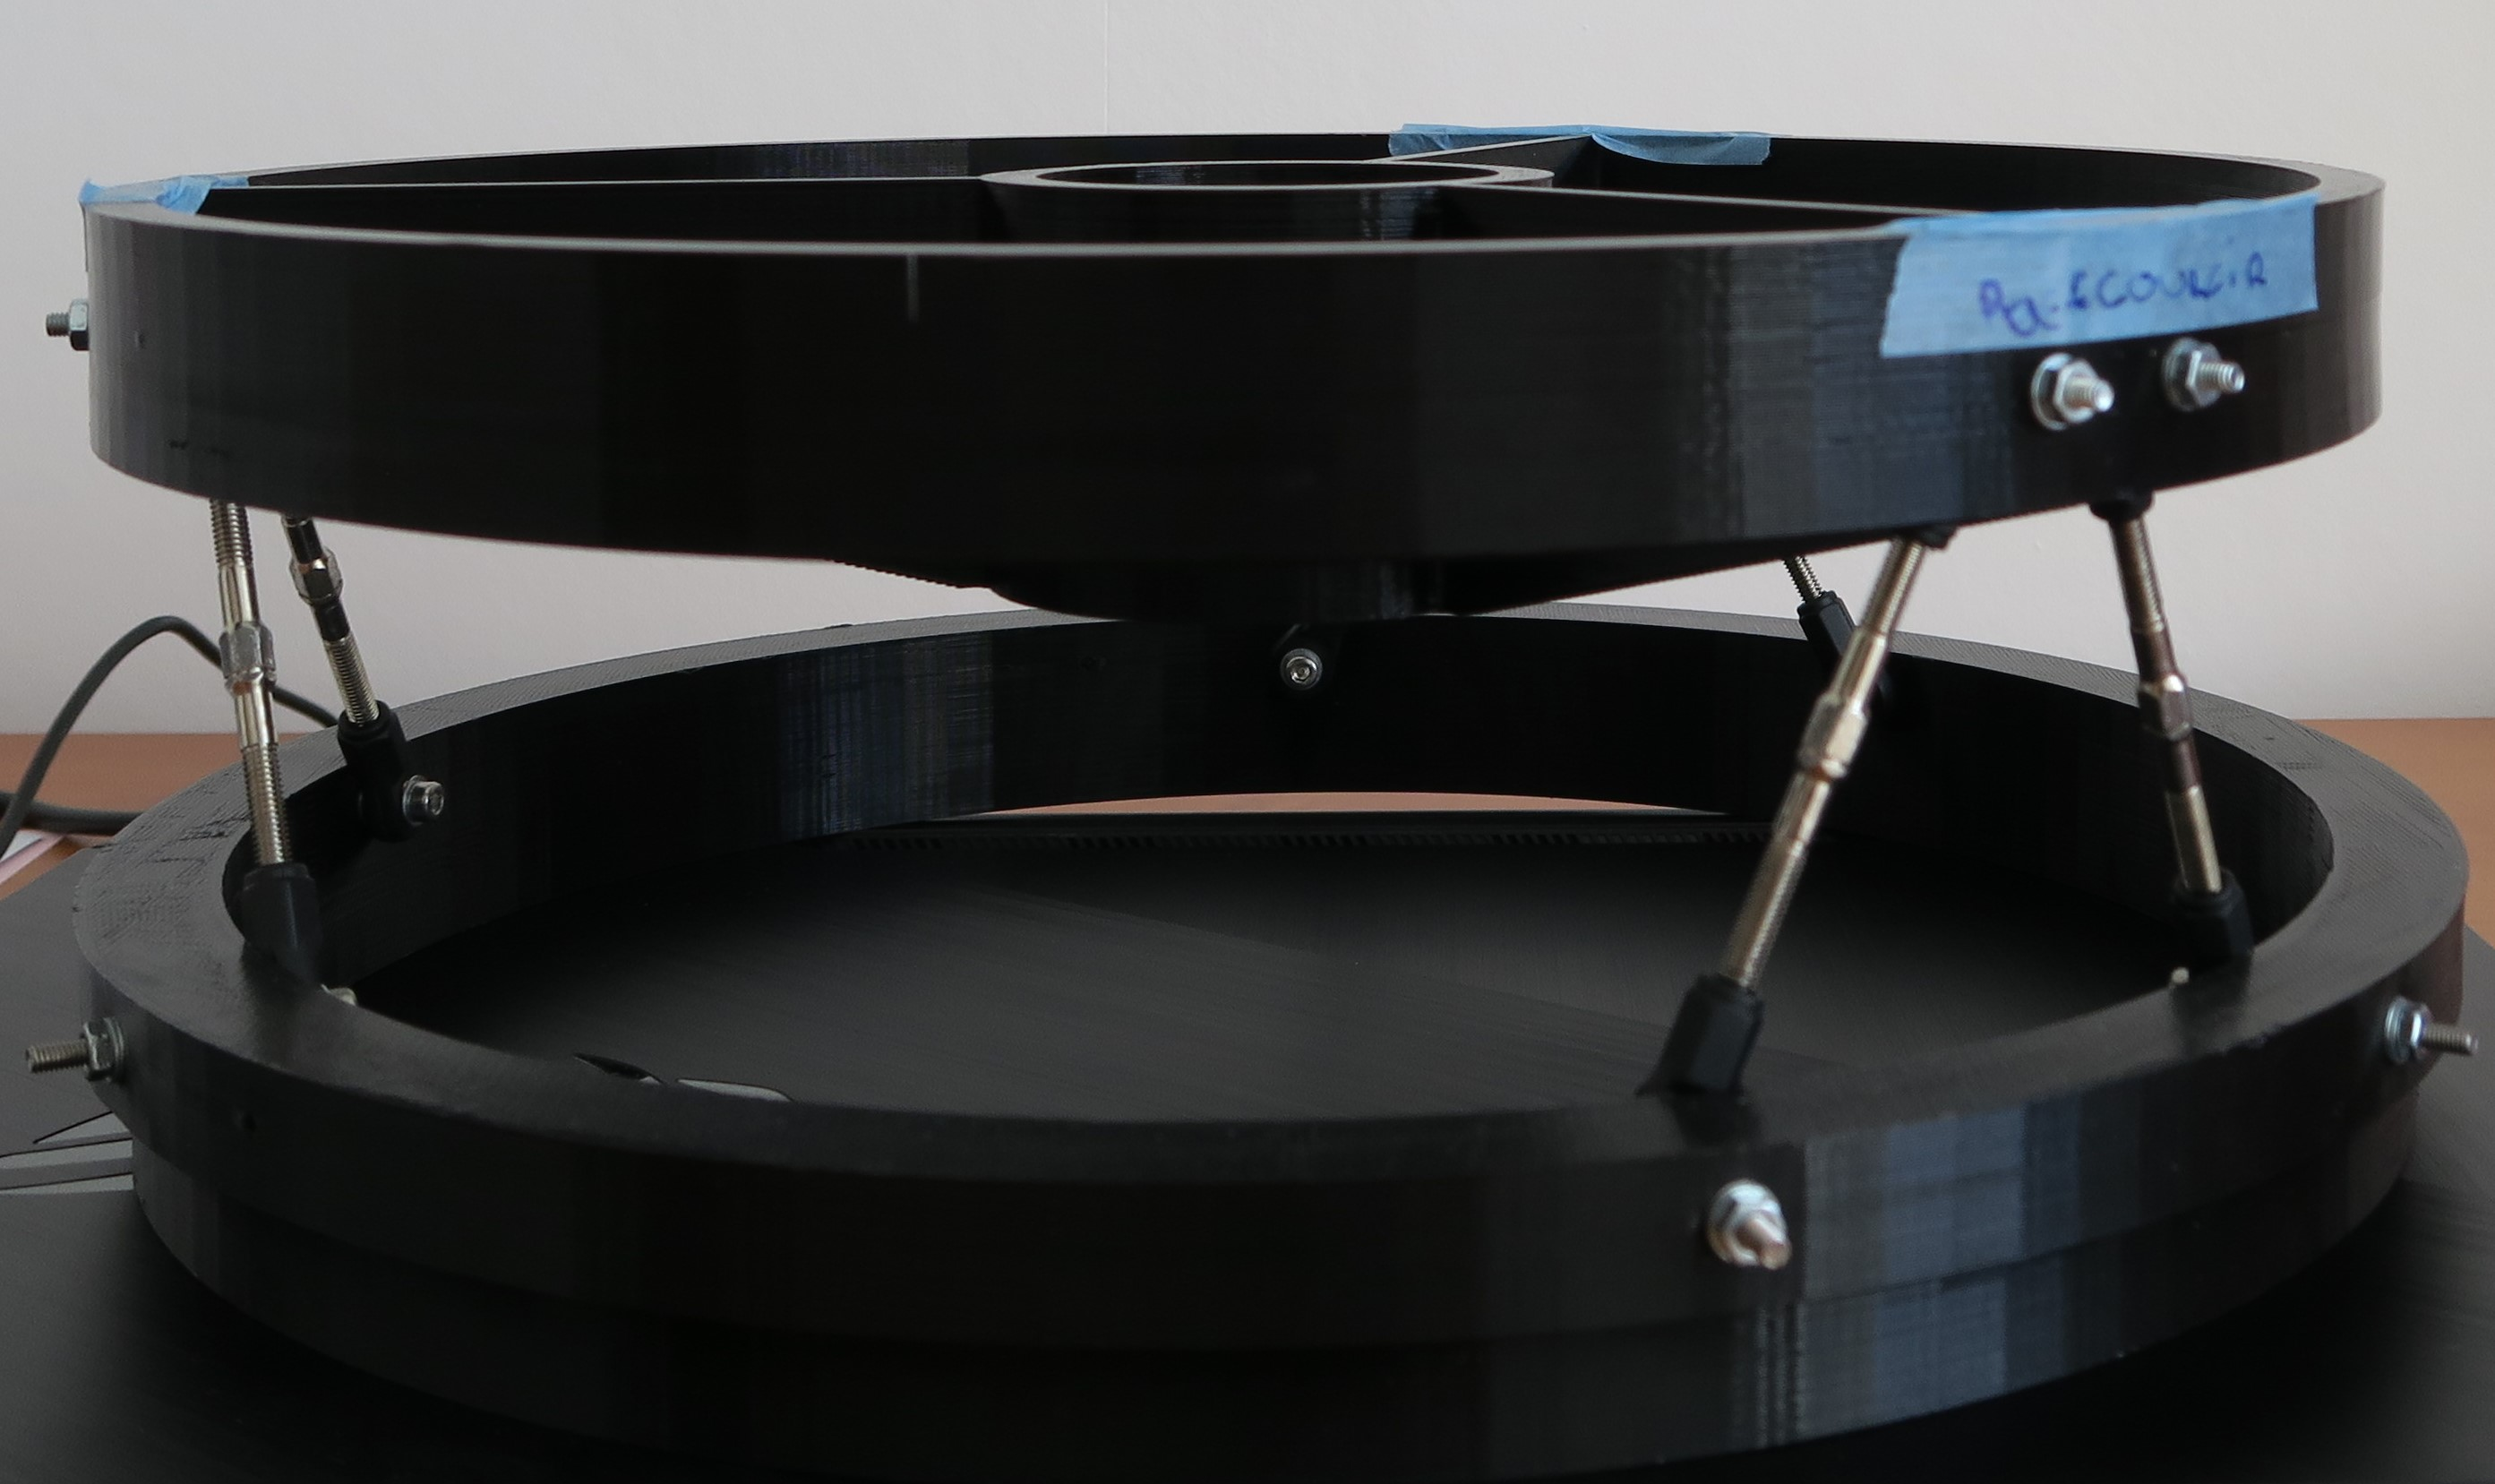
\includegraphics[width=\textwidth]{plateforme a niveau.jpg}
    \end{subfigure}
    \caption{Plateforme avant et après mise à niveau}
\end{figure}


Cela vient également en contradiction avec le tableur. En effet, le modèle théorique supposait que les six fixations des bielles sur le plateau bas étaient équidistantes. 
Cependant, le fait de repercer la plateforme pour répondre aux contraintes des bielles a faussé le tableur. 
Pour l'utilisation du modèle mathématique, nous avons donc mis une hauteur théorique, entre les deux plateaux, de cinquante millimètres et nous avons gardé un \og delta théta \fg \ de 30\degree.
Ces deux paramètres nous permettent néanmoins d'avoir un bon aperçu de l'utilisation du tableur.  

\begin{figure}[H]
  \centering
  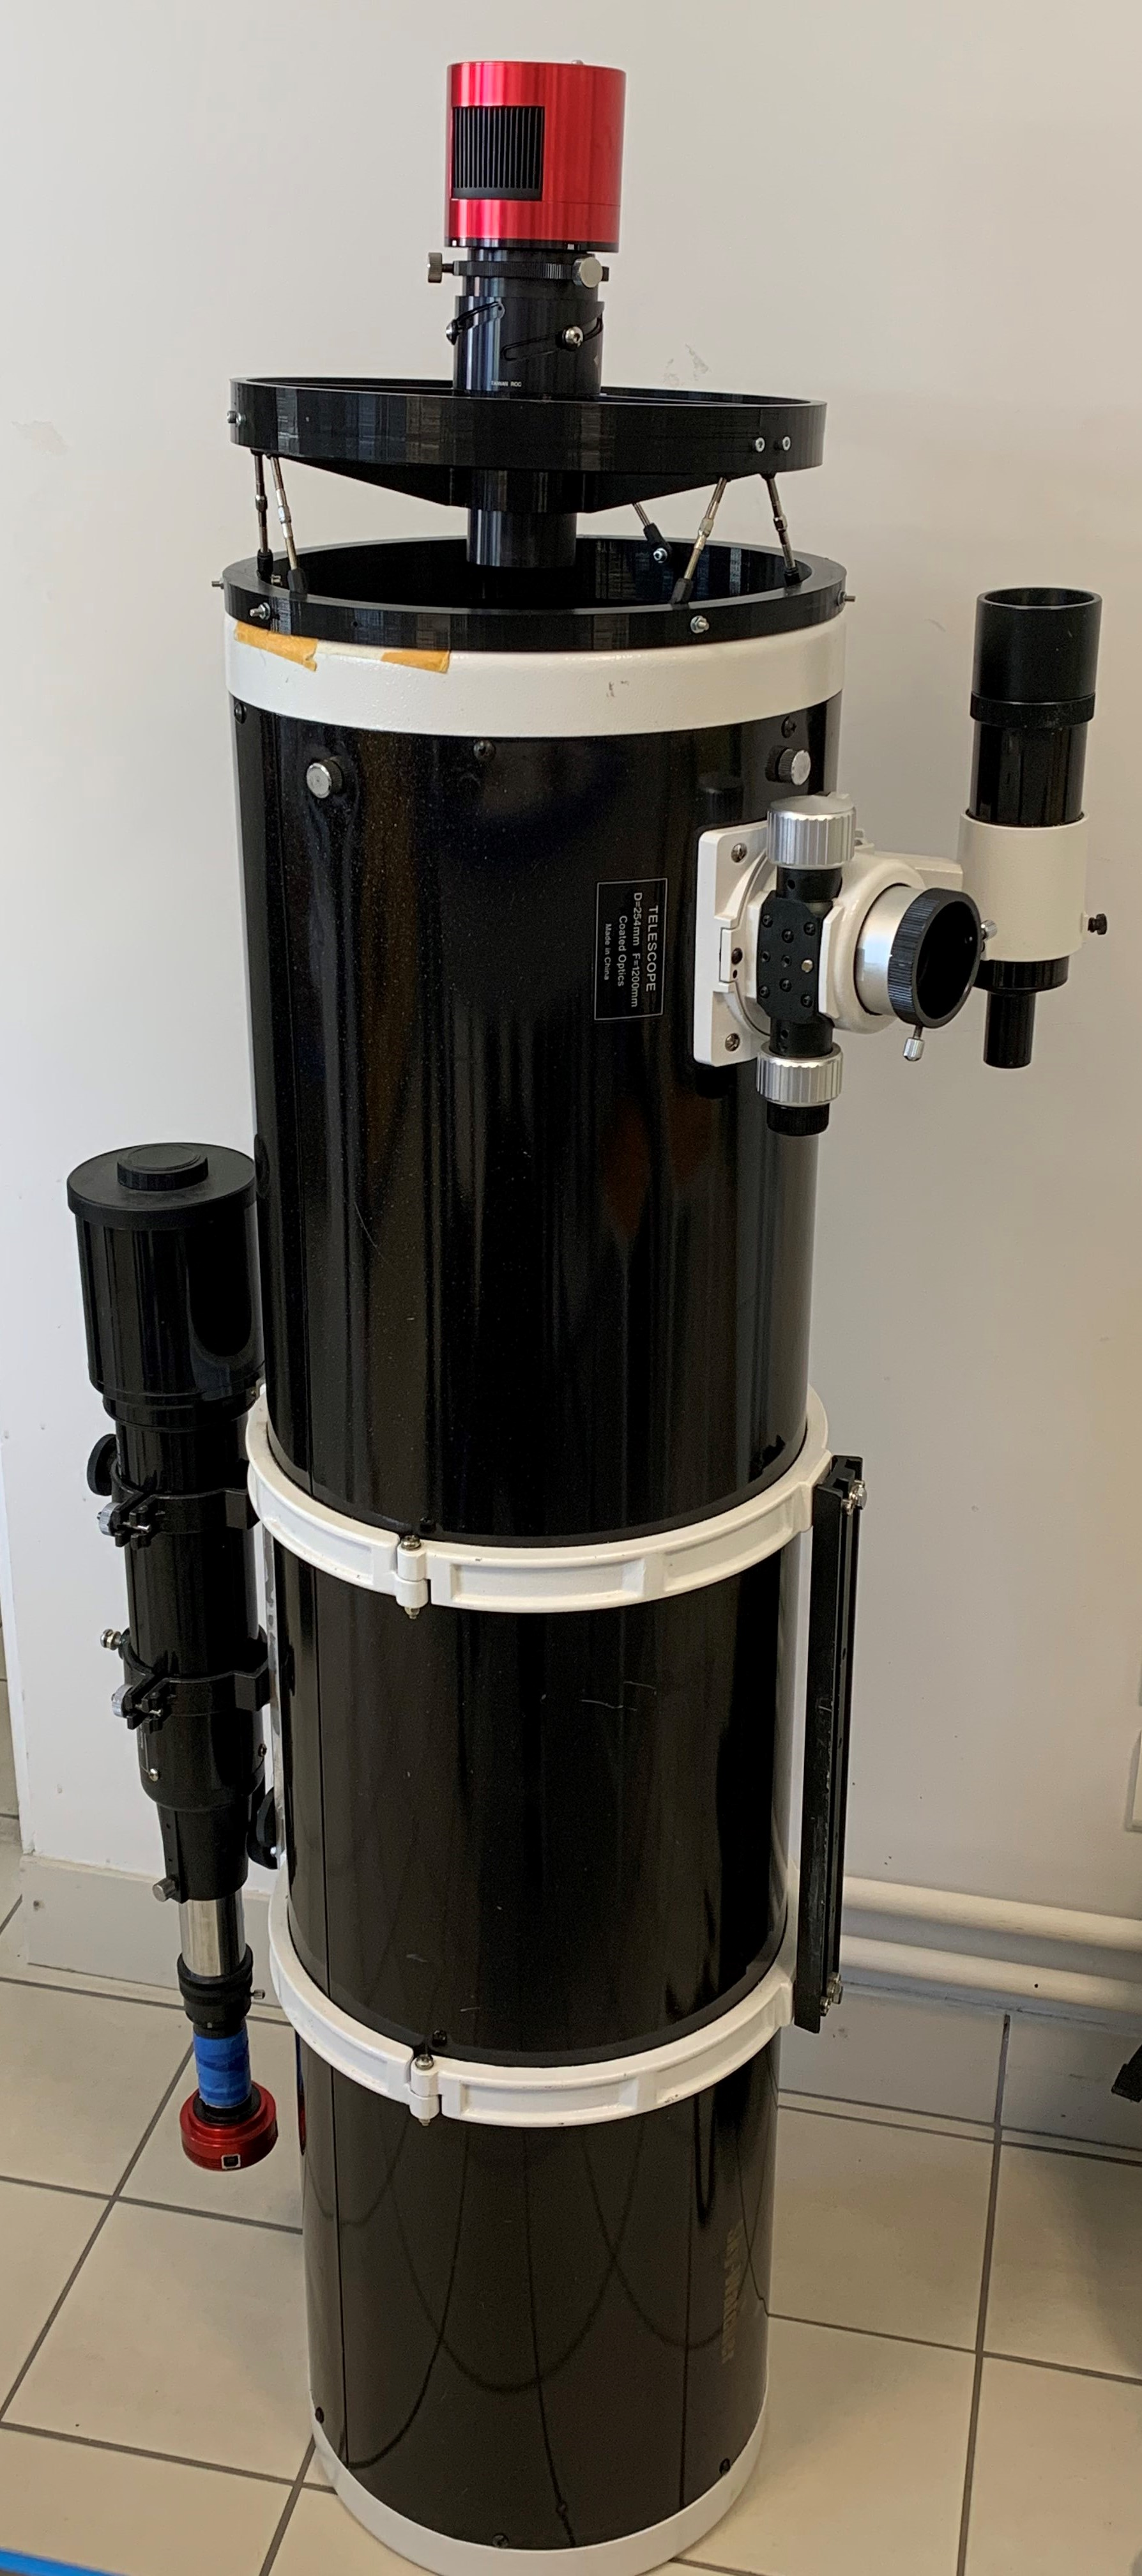
\includegraphics[width=0.25\textwidth]{telescope.jpg}
  \caption{Montage de la plateforme sur le télescope}
\end{figure}




\newpage

\section{Conclusions et perspectives}

Ce projet, notre premier projet, nous permet de mieux appréhender
ce qu’est le métier d’ingénieur. La durée de ce projet ainsi que sa complexité nous donnent un premier aperçu de ce à quoi nous serons confrontés dans notre activité professionnelle. Cette
première approche nous initie aussi aux différentes étapes d’un projet. Nous avons
commencé par une phase conséquente de compréhension et de visualisation du fonctionnement de la plateforme de Stewart. Cette phase a été la plus
longue. Ensuite, nous avons recherché les formules mathématiques adéquates aux
mouvements de la plateforme, cette partie du projet est celle qui a été la plus compliquée
étant donné nos connaissances scientifiques et nos compétences techniques à ce stade de notre cursus. Néanmoins, grâce à de très nombreux échanges avec Monsieur Bouzidi, nous sommes parvenus à créer le tableur contrôlant les positions de la plateforme.  C'était une étape nécessaire et obligatoire avant d'aborder celles de la modélisation et de la réalisation.
Pour finir, la dernière étape était celle l’assemblage afin d’obtenir une plateforme opérationnelle.
Nous avons réussi à tenir les temps malgré des délais plus serrés sur la fin du projet,
toujours accompagnés de notre encadrant qui nous l'a bien exposé et ensuite bien guidé dans ses différentes étapes.
Ce projet nous aura aussi permis de travailler en collectif et de nous responsabiliser individuellement (temps collectifs de coordination d'équipe en présentiel et distanciel, répartition des tâches à réaliser (réflexion/conception/modélisation/application concrète), co-rédaction du rapport). 

\medskip

La plateforme est exactement aux bonnes dimensions pour recevoir le télescope et le
plateau supérieur aux bonnes dimensions pour accueillir la caméra. La plateforme est solide
et répond au besoin auquel nous faisons face. Cependant, les bielles sont
très dures à manoeuvrer pour en modifier la longueur. De plus, ces bielles sont trop courtes et ne permettent pas un espace suffisant entre les deux plateaux. Enfin, la translation entre les deux plateaux fait que la caméra ne se trouve pas exactement au niveau du point focal.

\medskip

Malgré tout, nous sommes allés jusqu'à la fin de la conception/réalisation de la plateforme de Stewart et le modèle est viable. La plateforme pourrait trouver une amélioration en l'équipant de nouveaux actionneurs linéaires plus à même de s'adapter aux contraintes d'utilisation et au modèle mathématique. Pour aller encore plus loin, il serait possible de créer un programme qui réglerait la plateforme automatiquement à la bonne distance, afin de disposer  d'une plateforme autonome. Il faudrait pour cela l'équiper de vérins contrôlés par des servomoteurs.
Il ne nous reste plus maintenant qu'à  tester le télescope équipé de sa plateforme pour ensuite admirer les clichés.


\begin{figure}[H]
  \centering
  \includegraphics[width=0.35\textwidth]{Nebuleuse_dorion.PNG}
  \caption{Nébuleuse d'Orion (Nicolas Dupont-Bloch - \url{http://nicolas.dupontbloch.free.fr}
)}
\end{figure}

\newpage

\section{Remerciements}

Nous tenons à remercier notre encadrant, Monsieur Rabah Bouzidi, pour le temps qu'il nous a consacré tout au long du projet, ses explications, sa disponibilité et ses conseils. Nous le remercions également de bien avoir voulu imprimer la plateforme avec son équipement personnel, sans quoi le projet n'aurait pas abouti. 

\medskip

Nous remercions également Monsieur Cédric Doutriaux, responsable du FabLab, pour ses conseils, notamment quant à l'utilisation de FreeCAD, et sa disponibilité pour répondre à nos questions tout au long du projet.

\medskip

Pour finir, nous remercions Monsieur Nicolas Dupont-Bloch qui a été à l'origine de ce projet et qui nous a accordé le droit d'utiliser une de ses photos du ciel profond. (\url{http://nicolas.dupontbloch.free.fr})



\newpage
\section{Références}

Comme mentionné dans le rapport, ce projet a pris forme grâce aux très nombreux échanges que nous avons eu avec Monsieur Bouzidi, également ceux avec Monsieur Doutriaux. 
C'est pourquoi nous n'avons utilisé que peu de ressources externes. 
Voici toutefois les références utilisées durant le projet pour appréhender le fonctionnement de la plateforme de Stewart : 
\newline
-\url{https://www.xarg.org/paper/inverse-kinematics-of-a-stewart-platform/} 
\newline
-\url{http://www.scielo.br/scielo.php?script=sci_arttext&pid=S1678-58782012000200011}
\newline
-\url{https://www.3sigma.fr/Systemes_didactiques-Commande_de_la_plateforme_de_Stewart_Deltalab.html} 
\newline
-\url{https://fr.wikipedia.org/wiki/Plateforme_de_Stewart}

\bigskip

Voici le lien permettant d'accéder aux bielles que nous avons utilisées pour le montage de la pateforme :
\newline
\url{https://www.conrad.fr/p/barre-darticulation-reely-538057-1-pcs-1301679}

\bigskip

Voici l'accés au site internet de Monsieur Dupont-Bloch : 
\newline
\url{http://nicolas.dupontbloch.free.fr}

\bigskip

Vous trouverez tous nos documents sur le dépôt GitHub dont voici le lien :
\newline
\url{https://github.com/simonmsd/Plateforme-Stewart.git}



\bibliographystyle{plain}
\bibliography{CMIbib}




\end{document} 


